\newif\ifdraft\drafttrue  % set true to show comments
\newif\ifplentyoftime\plentyoftimefalse  % :-)

\documentclass[acmsmall,review,anonymous]{acmart}\settopmatter{printfolios=true,printccs=false,printacmref=false}
% % For double-blind review submission, w/ CCS and ACM Reference
% \documentclass[acmsmall,review,anonymous]{acmart}\settopmatter{printfolios=true}
% % For single-blind review submission, w/o CCS and ACM Reference (max
% submission space)
% \documentclass[acmsmall,review]{acmart}\settopmatter{printfolios=true,printccs=false,printacmref=false}
% % For single-blind review submission, w/ CCS and ACM Reference
% \documentclass[acmsmall,review]{acmart}\settopmatter{printfolios=true} % For
% final camera-ready submission, w/ required CCS and ACM Reference
% \documentclass[acmsmall]{acmart}\settopmatter{}


% % Journal information % Supplied to authors by publisher for camera-ready
% submission; % use defaults for review submission.
\acmJournal{PACMPL}
\acmVolume{1}
\acmNumber{ICDP} % CONF = POPL or ICFP or OOPSLA
\acmArticle{1}
\acmYear{2018}
\acmMonth{1}
\acmDOI{} % \acmDOI{10.1145/nnnnnnn.nnnnnnn}
\startPage{1}

% % Copyright information % Supplied to authors (based on authors' rights
% management selection; % see authors.acm.org) by publisher for camera-ready
% submission; % use 'none' for review submission.
\setcopyright{none}
\usepackage{amsmath, amssymb, verbatim, enumerate, graphicx, centernot, tikz,
array, mathtools, bussproofs, stmaryrd, enumitem, stackengine, subcaption}
\captionsetup{compatibility=false}
\usepackage{relsize}
\usepackage{listings}
\usepackage{proof}


\lstset{
language=Caml, basicstyle=\upshape\sffamily,
keywordstyle=\upshape\sffamily\color{dkblue}, keepspaces=true,
framexleftmargin=1ex, framexrightmargin=1ex, showstringspaces=false,
commentstyle=\itshape\rmfamily, columns=flexible,
% BCP: I find this distracting:
% stringstyle=\sffamily\color{dkred},
mathescape
}

% %%%% Macros Colors
\definecolor{dkblue}{rgb}{0,0.1,0.5}
\definecolor{dkgreen}{rgb}{0,0.6,0}
\definecolor{dkred}{rgb}{0.6,0,0}
\definecolor{dkpurple}{rgb}{0.7,0,0.4}
\definecolor{olive}{rgb}{0.4, 0.4, 0.0}
\definecolor{teal}{rgb}{0.0,0.5,0.5}
\definecolor{orange}{rgb}{0.9,0.6,0.2}
\definecolor{lightyellow}{RGB}{255, 255, 179}
\definecolor{lightgreen}{RGB}{170, 255, 220}
\definecolor{teal}{RGB}{141,211,199}
\definecolor{darkbrown}{RGB}{121,37,0}

\newcommand{\FINISH}[3]{\ifdraft\textcolor{#1}{[#2: #3]}\fi}
\newcommand{\bcp}[1]{\FINISH{dkred}{B}{#1}}
\newcommand{\BCP}[1]{\FINISH{dkred}{B}{\bf #1}}
\newcommand{\afm}[1]{\FINISH{dkgreen}{A}{#1}}
\newcommand{\dpw}[1]{\FINISH{dkblue}{D}{#1}} % Toronto Maple Leafs Blue :-)
\newcommand{\saz}[1]{\FINISH{orange}{SZ}{#1}}
\newcommand{\ksf}[1]{\FINISH{teal}{K}{#1}}
\newcommand{\sam}[1]{\FINISH{dkpurple}{SM}{#1}}

% For Inference Rules
\newcommand{\Rule}[2]{\infer{#2}{#1}}
\newcommand{\RuleSide}[3]{\infer[#3]{#2}{#1}}
% \newcommand{\Axiom}[1]{\Rule{}{#1}}

\newcommand{\wf}[1]{\ensuremath{#1\;\mathsf{wf}}}

% FOR Regular Expression names
\newcommand{\re}[1]{\ensuremath{\mathtt{#1}}}
\newcommand{\kw}[1]{\ensuremath{\mathsf{#1}}}
\newcommand{\codefont}[1]{\ensuremath{\mathsf{#1}}}
\newcommand{\project}[2]{\ensuremath{\kw{project} \; #1 \mapsto #2}}
\newcommand{\squash}[3]{\ensuremath{\kw{squash} \; #1 \rightarrow #2
\kw{using} \; #3}}
\newcommand{\perm}[2]{\ensuremath{\kw{perm}\; (#1)\; \kw{with}\; #2}}
\newcommand{\normalize}[3]{\ensuremath{\kw{normalize} \; (#1, #2, #3)}}
\newcommand{\sep}{\ensuremath{\ | \ }}
\newcommand{\canonizer}{\ensuremath{\kw{Canonizer}}}
\newcommand{\bibtex}{\textsc{Bib}\TeX{}}
\newcommand{\get}{\ensuremath{\kw{get}}}
\newcommand{\semicolon}{\ensuremath{\; ; \;}}
\newcommand{\lput}{\ensuremath{\kw{put}}}
\newcommand{\create}{\ensuremath{\kw{create}}}
\newcommand{\eqrel}[1]{\ensuremath{\equiv_{#1}}}

\newcommand{\Name}{Optometrist}

\newcommand{\QRESize}{\textbf{QS}}
\newcommand{\CanonizerAndSpecSize}{\textbf{CS}}
\newcommand{\LensAndSpecSize}{\textbf{LS}}

\newcommand{\OpticianRuntime}{\textbf{OO}}
\newcommand{\SystemOnOptician}{\textbf{SO}}
\newcommand{\SystemOnBenchmarks}{\textbf{SS}}
\newcommand{\cd}[1]{\lstinline[backgroundcolor=\color{white}]$#1$}


% %%%%%%%%%%%%%%%%%%%%%%%%%%%%%%%%%%

\begin{document}
\title{Synthesizing Quotient Lenses}
\begin{abstract}
\saz{The old abstract read more like an introduction, so we modified it to be
the ``new'' introduction.}
\end{abstract}

\keywords{quotient lenses, synthesis}
\maketitle              % typeset the title of the contribution

\section{Introduction}

Oftentimes, the same data is stored in a variety different formats. For
example, \bibtex{} and EndNote both store bibliography data; spreadsheet data
can be represented as a CSV file or a TSV file; web APIs can return data as a
JSON or
XML object. When different applications manipulate data in different formats,
synchronizing the applications amounts to synchronizing their respective data
formats. One way to synchronize data formats is to use \emph{lenses}, \emph{i.e.,} programs that represent pairs of functions for translating data from
format A to B (the \emph{get} direction) and back again (the \emph{put}
direction).  These lenses, when defined using domain-specific
languages like Boomerang~\cite{boomerang} or
BiGul~\cite{DBLP:conf/pepm/KoZH16}, typically come with a variety of guarantees,
the \emph{lens laws}, that help ensure put and get functions are effective
inverses of one another.
%comprise such synchronization functions, and the ``lens
%laws'' provide restrictions on how these synchronization functions interoperate%.
%Bidirectional languages like Boomerang~\cite{boomerang} and
%BiGul~\cite{DBLP:conf/pepm/KoZH16} use a single expression to encode all of the
%lens's synchronization functions at the same time.

One way to classify lenses is by the laws they obey.  Amongst the most
restrictive lenses are the \emph{bijective lenses}.  These lenses demand
that get and put functions for a bijection, meaning no information
is lost when one translates from data format to another.  While this
strong guarantee can be useful in some contexts, it is more often the case
that some of the information in one or both of the data formats is superfluous.
For instance, one typically does not care to preserve the amount of
whitespace between characters.  In other circumstances, capitalization
or the order of fields in a record or items in a list may be unimportant.
%
%bijective lenses have
%strong correctness guarantees, they are often
%However, these lens laws are too restrictive for many important transformations.
In particular, these lens laws do not permit transformations that put the data
in canonical forms.
For instance, to return to our bibliography example, in \bibtex{},
an author can be specified as
``\cd{lastname, firstname}'' or as ``\cd{firstname lastname}''---it does not matter which of the
two formats is used.
%While it is important to allow authors
%to be input in both ways, we would like these authors to only be output as
%\cd{firstname lastname}, but the lens laws prevent such functions.
{\em Quotient lenses}~\cite{quotientlenses} loosen many of the restrictions
of bijective lenses by introducing an equivalence relation and considering
bijections modulo that relation.  Such quotient lenses make it possible
to align many more data sources than would otherwise be possible by
ignoring details that a programmer views as inessential.
%each of the data formats is quotiented by some equivalence relation and the lens
%laws are taken modulo equivalence.
%This allows lenses to be simpler and more
%flexible. For example, inessential details like whitespace and orderings of
%fields can be ignored when writing the transformations between the formats.

%However, while plain lenses are widely used in both standalone systems and
%popular libraries, Boomerang~\cite{boomerang} is the only implementation
%currently offering quotient lenses. Even though quotient lenses permit simpler
%transformations between the formats, they merely push complexity elsewhere.
Ordinary bijective lenses are fairly tricky to program, especially for
beginners, as they require programmers to think in two directions at once
and learn a new type system, which comes with some tricky ambiguity constraints.
Unfortunately, quotient lenses do not improve the situation:  To
write a quotient lens in Boomerang, programmers must work with standard lens
combinators as well as a system of \emph{canonizers}.
These canonizers encode two functions, one that
maps data represented in the original external format
to a canonical element, and another, in the opposite direction, that chooses
which elements of the original format correspond to values in the canonical
format. Furthermore, if a user wants to define the domain and range of
a lens explicitly (a programming practice that is encouraged), she must
provide regular expressions defining input and output formats.
Consequently, to define a quotient lens, one must often three different sorts
of terms: (1) regular expressions that define the two data formats
to be processed, (2) canonizers to normalize the data
and choose representatives, and (3) a bijective lens maps
one canonical form into another.  Somewhat frustratingly,
these three terms share a fair amount of structure.
%Moreover, writing the lens between the equivalence classes can be
%challenging due to the rather fiddly typechecking, mainly due to
%``non-ambiguity'' conditions in the lens well-formedness rules.

In this paper, we improve the process of programming quotient lenses
in two distinct, but connected ways. First, we
introduce a new language of {\em Quotient Regular Expressions}, or QREs, which
enable a programmer to simultaneously specify a regular expression as well as
a set of canonical representatives for strings that match the regular
expression. With
QREs, programmers do not need to define the data and canonization functions
separately -- by adding simple annotations to ordinary regular expressions,
canonization functions can be inferred.

Second, we use QREs to define a class of quotient lenses called {\em QRE
lenses}, and, we show how to synthesize such QRE
lenses automatically.  
More specifically, in
order to generate a lens, a programmer provides a pair of QREs
describing the source and target formats, and, optionally,
a suite of examples that demonstrates how the
lens should act on specific examples.  Given this information,
we are able to exploit and extend recent work on algorithms for synthesis of
bijective lenses~\cite{optician} to generate quotient lenses.
Importantly, the lenses generated by
our synthesis algorithm are guaranteed to translate data back and forth
between source and target QREs and to satisfy the provided examples.
Moreover, while our synthesized quotient lenses have a relatively
restricted form (a fact that cuts down the amount of non-determinism in
a specification and thus helps speed up synthesis), we prove that
this rigidity does not compromise expressiveness.

The following list summarizes the central contributions of our work.
\begin{enumerate}
  \item We introduce {\em Quotient Regular Expressions} (QREs)
  which provide a compact, convenient notation that expresses an equivalence
  relation on a regular languages as well as a canonical set representatives
  for this equavalence relation (Section~\ref{QRE}).
  \item We define a language of {\em QRE lenses}.  This language is
  a subset of the bijective quotient
  lenses whose types are given by QREs. Our main technical contribution
  is a proof that each QRE lens $q$ defines the same transformation as a
  QRE lens $q'$ that is in normal form. (Section~\ref{QRE-lenses}).
  \item Using this normal form, we reduce the problem of {\em synthesizing}
  QRE lenses to the previously studied problem of synthesizing bijective lenses
  between regular languages (Section~\ref{synth}).
  \item We extend the Boomerang {\em implementation} with QREs
  and QRE lens synthesis.  We demonstrate the utility of our
  implementation by using it to
  synthesize QRE lenses between several real-world data formats from the
  {\tt data.gov} database (Section~\ref{impl}).
\end{enumerate}
Sections~\ref{relwork} and~\ref{concl} discuss related and future work.

\section{Quotients by Example}
\label{sec:example}

%In this section, we explain the difficulties of programming with quotient
%lenses in Boomerang and show, by way of example, how our 
%{\em Quotient Regular Expressions} (QREs) help alleviate these difficulties.

\emph{Lenses} define computations that can be read in two directions, forwards and
backwards.  The simplest lenses define bijections between source and
data, but we are interested in \emph{quotient lenses}, which define
bijections modulo some equivalence relation.  The remains of this section
describe and motivate a new language and system for defining such lenses.

To begin, consider a bidirectional transformation that converts
\bibtex{} citation records such as
\begin{verbatim}
@Book {conway,
Author = "J. H. Conway",
Title = {Regular Algebra and Finite Machines}
}
\end{verbatim}
\noindent
into an equivalent EndNote format like the following
\begin{verbatim}
%0 Book
%T Regular Algebra and Finite Machines
%A J. H. Conway
%F conway
\end{verbatim}
\noindent
and vice versa.
%
Notice that transformations from one format to the other preserve
most of the information present in the data:  the title, the author,
and the key, for instance.  However, some information in the syntax
may be lost.  For instance, users are typically uninterested in preserving
the amount of the whitespace between words or
between fields.  The order of author and title fields is also likely
irrelevant and there may be equivalent ways of writing the same
name:  ``Conway, J. H.'' vs ``J. H. Conway.''

%% Moreover,
%% if two \bibtex{} files differ only in ``inessential'' details, we would like
%% to treat them the same by mapping them to identical EndNote representations.
%% In this , the transformation should allow whitespace characters to occur
%% arbitrarily between the words in the label, author, and title fields, as well as
%% in between them. Second, an author's name can have the surname followed by a
%% comma and then the other names separated by arbitrary whitespace, or just all
%% the names separated by arbitrary whitespace (for example, the names ``Conway, J.
%% H.'' and ``J. H. Conway'' are equivalent). Lastly, the transformation should
%% also ignore the order in which the author and title fields occur in each
%% citation record.

When two instances of the same format differ only terms of such inessential
information, it is often useful to treat them as identical and to map them
into canonical representations.
Continuing our example, the following two
\bibtex{} citations represent the same logical object and as a result, should
be translated to the same EndNote record.
\begin{verbatim}
@Book {conway,
Author = "J. H. Conway",
Title = {Regular Algebra and Finite Machines},
}

@Book{     conway,
Title = {Regular Algebra
and Finite Machines},
Author = "Conway, J. H.",     }
\end{verbatim}

One natural way to define lenses that will synchronize data in these formats
is to provide the following items:

\begin{enumerate}
\item A pair of descriptions of the external source and target formats.
Such descriptions may be given by regular expressions, for instance.
They serve as documentation to describe the domains over which the lens
is to operate.
\item A pair of \emph{canonizers} that map external source (and target)
objects into internal, canonical forms.  Such canonizers will take
care of stripping away irrelevant information and otherwise normalizing
differences between equivalent representations of the same logical data.
When given an internal representation, such canonizers must also operate
in the reverse direction, \emph{choosing} an element in the external format
to represent the canonical internal element.
\item A pair of descriptions of the internal source and
target formats, again, to document the structure of the transformation.
\item A bijective lens to map back and forth between canonical elements
of the internal source and target formats.
\end{enumerate}

\noindent
Indeed, Boomerang's quotient lenses are structured this way~\ref{boomerang}.
Of course, some of these elements are optional.  For instance, it is
not necessary to document internal and external formats.  However, we do
view it as good engineering practice to do so, as such documentation makes
lenses easier to read, understand, use and maintain.  In this case, there is
significant redundancy here:  External and internal formats
typically have some overlap; external formats and canonizers have related
structure; and the structure of bijective lens computations is largely driven
by the structure of the internal formats.  Hence, overall, a more compact
notation would simplify description and legibility of such computations.
In addition,
the lens and canonizer languages themselves can be somewhat fiddly and
difficult to
master.  For instance, to quotient out whitespace inside, and in between,
fields while also ignoring field order one must nest canonizing combinators
within one another in a somewhat tricky and fiddly way.  

%% %Foster's Boomerang~\ref{boomerang} language presents one design
%% While it is possible to express the equivalence on the \bibtex{} data above in
%% Boomerang, actually doing so is a challenge.  Three of the inessential details
%% we wish to ignore---whitespace quotienting
%% inside fields, whitespace quotienting in between fields, and permutation
%% quotenting of fields---nest within each other in a way that makes them difficult
%% to express with the existing Boomerang combinators. Furthermore, if the
%% programmer wishes to specify the type of the lens, then she can only specify
%% data formats on each side of the lens with a regular expression that does not
%% keep track of the equivalence relation defined on the language of the regular
%% expression. Consequently, the programmer has to write a regular expression as
%% well as a canonizer that expresses the equivalence relation on that regular
%% expression, even though a regular expression and the canonizer defined on it
%% typically share much of the syntactic structure. Having to write both of these
%% expressions makes programming with quotient lenses verbose and time consuming.

We propose to do away with much of this overhead, and the burden of a
fiddly programming process, by defining a single new compact notation
to specify data formats modulo an equivalence relation and then by
synthesizing the lenses that map between these formats automatically.

\subsection{Quotient Regular Expressions}

A {\em Quotient Regular Expression} (QRE) defines an external regular
expression $R$, an equivalence relation $\sim$ on the language
described by $R$, and a canonical set of representatives of $\sim$,
all at once.  QREs are constructed from a simple set of primitives
and composed using familiar regular operators
(choice `\cd{|}', concatenation `\cd{.}', sequential composition ``;''
and Kleene star `$^*$').

For example, to begin construction of our \bibtex{} format, we might
first define a whitespace format, which, externally, matches
any non-zero number of whitespace characters, and converts
any such whitespace into a single space character (its canonical form).
Such a definition uses the \kw{project} primitive to implement the
specification:

\begin{lstlisting}
let wsp = project [ \n\t\r]$^+$ $\to$ " "
\end{lstlisting}

While a projection chooses a single canonical representative for all elements
of a regular language, the \kw{squash} combinator maps data from one
regular language to another via a user-defined
function.  For instance,
if \codefont{comma_name} describes the format for ``Conway, J. H.''
and \codefont{space_name} describes the format for ``J. H. Conway''
and \codefont{s_to_c} is a function from one to the other then
the following instance of squash creates the desired canonizer.

%Figure~\ref{fig:example-qre} illustrates
%how to specify \bibtex{} records and their canonical elements using
%QREs.

\begin{lstlisting}
let name = squash comma_name $\to$ space_name using s_to_c
\end{lstlisting}

One way to define the function used by squash is simply to write it
from scratch in OCaml.  However, our system will also synthesize
such functions automatically from pairs of regular languages and
examples.
%
\begin{lstlisting}
let l = synth comma_name $\Leftrightarrow$ space_name using {("Conway, J. H.", "J. H. Conway")}
let s_to_c = get l
\end{lstlisting}
%
The first line above synthesizes a \emph{bidirectional} lens between
\codefont{comma_name} and \codefont{space_name} using the listed example
transformation as a guide.  The second line simply
extracts the left-to-right transformation from the lens, which is what we need for squash.

A third useful QRE primitive is the permutation combinator.  For example,
the following instance of \kw{perm} allows label, author and title fields
(which we assume have been defined earlier) to appear in any order.
%
\begin{lstlisting}
let bib_fields = perm (label, bib_author, bib_title) 
\end{lstlisting}
%
To normalize any repeated separator between fields, one can extend a permutation
with any other QRE.  For instance, below, we normalize whitespace between fields,
leaving only a single newline.
%
\begin{lstlisting}
let bib_fields = perm (label, bib_author, bib_title) with (project ("," .wsp$^+$) $\to$ ",\n")
\end{lstlisting}
%
\noindent
The QRE for the bibtex format is presented in its entirety in Figure~\ref{fig:example-qre}.


\begin{figure}[t]
\begin{lstlisting}
(* whitespace with " " as a canonical representative *)
let wsp = project [ \n\t\r]$^+$ $\to$ " "

(* define name representations with a space and with a comma *)
let space_name = name | (name . wsp . (name . wsp)$^*$ . name)
let comma_name = name | (name . "," . wsp . (name . wsp)$^*$ . name)

(* synthesize a lens that maps the comma representation to the space representation *)
let space_to_comma = synth comma_name $\Leftrightarrow$ space_name using {("Conway, J. H.", "J. H. Conway")}

(* squash QRE maps comma_name to space_name *)
let name = squash comma_name $\to$ space_name using (get space_to_comma)

(* define rest of bibtex fields *)
let name_sep = wsp . "and" . wsp
let bib_names = name | (name . name_sep . (name . name_sep)$^*$ . name)
let bib_author = "author = \"" . bib_names . "\""
let title = word | (word . wsp . (word . wsp)$^*$ . word)
let bib_title = "title = {" . title . "}"

(* allow any permutation of fields interspersed with arbitrary whitespace *)
let bib_fields = perm (label, bib_author, bib_title) with (project ("," .wsp$^+$) $\to$ ",\n")
let bibtex = "@book{" . bib_fields . "}"
\end{lstlisting}
\caption{QRE specification of \bibtex{} records. }
\label{fig:example-qre}
\end{figure}

%% In Figure~\ref{fig:example-qre}, the QRE \verb+project [ \n\t\r]+$^{+} \to$
%% \verb+" "+ matches any non-zero number of whitespace characters and quotients
%% them to a single equivalence class with a single space as the canonical
%% representative. We call this QRE a \textit{projection} because an entire regular
%% language is projected to a single representative string.

%% Another QRE in Figure~\ref{fig:example-qre} is given by

%% \begin{center}
%% \begin{lstlisting}
%% squash comma_name $\to$ space_name using (get space_to_comma)
%% \end{lstlisting}
%% \end{center}

%% \noindent This QRE is a \textit{squash} QRE. A \textit{squash} QRE ``glues''
%% two data formats using a user-defined function. For example,
%% the QRE in the code above specifies that the \cd{comma_name} representation of
%% the author's name is equivalent to the \cd{space_name} representation, with
%% \cd{space_name} taken to be the canonical representation. The
%% function that identifies the two formats is given by \cd{get space_to_comma},
%% which transforms names in the \cd{comma_name} representation to names in the
%% \cd{space_name} representation. In this example, \cd{space_to_comma} is itself
%% an automatically \textit{synthesized} lens between the \cd{space_name} and
%% \cd{comma_name} QREs, and we need to use the ``get'' direction of the lens to
%% specify the squash transformation.

%% The third example of a QRE in the Figure is \cd{bib_fields}, defined by:
%% \begin{center}
%% \begin{lstlisting}
%% perm (label, bib_author, bib_title) with (project ("," . wsp$^+$ ) $\to$ ",\n")
%% \end{lstlisting}
%% \end{center}

%% \noindent This is a \textit{permutation} QRE that specifies that the label,
%% title, and author fields can occur in any order, with the fields separated by a
%% comma followed by arbitrary amounts of whitespace. The canonical representation
%% is that in which the label, author and title fields occur in that order,
%% separated by a comma followed by a newline. The \textit{permutation} QRE is
%% designed for equivalences such as this, where different permutations of
%% equivalences are interspersed with a separator which itself has an
%% equivalence defined on it.

%% Given the \textit{projection}, \textit{squash}, and \textit{permutation}
%% QRE primitives, we can build more complex languages using the usual regular
%% expression combinators of alternative choice `\cd{|}', concatenation `\cd{.}'
%% and Kleene star `$^*$', and also sequential composition ``;''.

\subsection{QRE Lenses}
While QREs make it easier to write equivalence relations on regular expressions
by specifying the data and the equivalence relation on the data in one
expression, in order to define a quotient lens, the programmer still has to
manually derive the underlying lens that maps the equivalence classes of the
source data to the equivalence classes of the target data. This is itself a
tricky task as Figure~\ref{fig:example-lens} illustrates.

\begin{figure}[t]
\begin{lstlisting}
let preamble : (lens in "@book{" $\Leftrightarrow$ "%0 Book\n%F ") =
del "@book{" . ins "%0 Book\n%F "

let author_lens : (lens in (",\n" . bib_author) $\Leftrightarrow$ ("\n" . end_author)) =
del ",\nauthor = \""
. ins "\n%A "
. valid_name
. (del " and "
. ins "\n"
. (ins "%A " . valid_name . del " and " . ins "\n")$^*$ . ins "%A "
. valid_name
|| "")

let title_lens : (lens in ("\",\n" . bib_title . "},\n}") $\Leftrightarrow$ ("\n" . end_title)) =
del "\",\ntitle = {" . ins "\n%T " . title . del "},\n}"

let bib_to_end : (lens in bibtex $\Leftrightarrow$ end_note) =
preamble . label . author_lens . title_lens
\end{lstlisting}
\caption{An example lens between \cd{bibtex} and \cd{end_note} regular
expressions with no equivalences.}
\label{fig:example-lens}
\end{figure}

The lens shown in Figure~\ref{fig:example-lens} transforms \bibtex{} data to
EndNote data  (and vice versa) by matching the delimiters and separators in a
bijective manner. For example, the \cd{preamble} lens replaces the \bibtex{}
preamble \verb|@Book| with the EndNote preamble \verb|%0 Book\n%F|. When the
programmer is writing the lens, she has to make sure that all of these small
deletions and insertions are correct, which can be a challenging task if the
lens is large enough, as in the definition of the lens \verb!author_lens! in
Figure~\ref{fig:example-lens}. This makes lens programming tedious and
error-prone.

Consequently, we offer the programmer some relief by identifying a class of
quotient lenses that we call {\em QRE lenses}, and show how to {\em synthesize}
QRE lenses from a pair of QREs and a set of input-output example pairs. Our key
insight is to reduce the problem of synthesizing QRE lenses to the problem of
synthesizing {\em bijective lenses}~\cite{optician}, which are bijections created
from the Boomerang lens combinators.

QRE lenses lenses are the same as bijective lenses with ``canonizers at the
edges'' as in Figure~\ref{fig:attheedges}, and are typed using QREs---every QRE
lens $q$ has a type $q: c \Leftrightarrow c'$ where $c$ and $c'$ are QREs.
In the forward direction, a QRE lens $q: c \Leftrightarrow c'$ uses the source
QRE $c$ to compute a unique representative for the data modulo the equivalence
relation defined by $c$ and then applies the $\get$ function of a bijective
lens $\ell$ to this representative. In the backward direction, $q$ operates
similarly,  but using the view QRE $c'$ and the $\lput$ function of $\ell$.

\begin{figure}[t]
\centering
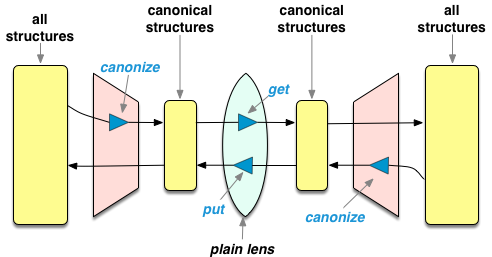
\includegraphics[width=\textwidth]{canonizers-outside}
\caption{Quotient Lens with ``Canonizers at the Edges''\sam{This is a
screenshot from Nate's thesis. Are we allowed to use it?}\bcp{We can
(if we put ``from [Nate's thesis]'' in the caption), but I don't think
we want the full complexity of asymmetric lenses here.  We should draw
the figure again.  (I have the OmniGraffle file for it, so this is
easy if I know how it should look.)}\bcp{Done---what do you think?}
\sam{Yes this is more accurate, except that we don't need a general choose
function. With QREs the kernel language is always contained in the whole
language so we just use the inclusion as the choose function.}}
\label{fig:attheedges}
\end{figure}

One potential pitfall with QRE lenses is that the combinators that we define on
them may not preserve this normal form. For example, the composition $q'; q$ of
QRE lenses $q$ and $q'$ might not be equivalent to any quotient lens that has
the canonical normal form of a bijective lens with canonizers at the edges.
Our main technical contribution in this paper is a proof that each QRE lenses
$q$ defines the same transformation as a QRE lens $q'$ that is in normal form.

For example, suppose \cd{q_1 : bibtex} $\Leftrightarrow$ \cd{endnote} is a QRE
lens that maps between \bibtex{} and EndNote formats, and that \cd{q_2 : endnote
<=> xml} is a QRE lens that maps between EndNote and XML formats. The
composition \cd{(q_1 ; q2) : bibtex} $\Leftrightarrow$ \cd{xml} of \cd{q_1} and
\cd{q_2} is not necessarily in normal form due to the presence of canonizers
on each side of the intermediary EndNote format:

\sam{TODO: We need to put a diagram of composition here.}

\noindent However, while \cd{q_1 ; q_2} is not in normal form, our main theorem
shows that there is another QRE lens \cd{q : bibtex} $\Leftrightarrow$ \cd{xml}
of the same type as \cd{(q_1 ; q2) : bibtex} $\Leftrightarrow$ \cd{xml} such
that \cd{q_1 ; q_2} and \cd{q} define the same transformation. This proof
will allow justify our approach for synthesizing quotient lenses so that the
programmer can replace all of the code in Figure~\ref{fig:example-lens} with a
call to the synthesis prodedure:

\begin{lstlisting}
let bib_to_end : (lens in bibtex $\Leftrightarrow$ endnote)
= synth bibtex $\Leftrightarrow$ endnote  using  {(bib_example, end_example)}
\end{lstlisting}
\noindent Here, the resulting  quotient lens maps between the \cd{bibtex} and
\cd{endnote} QREs, and sends the equivalence class of \cd{bib_example} to
the equivalence class of \cd{end_example}, which are the two concrete example
strings given at the beginning of this Section.

As we saw with the definition of \cd{space_to_comma} in
Figure~\ref{fig:example-qre}, the synthesis procedure itself can be used to
create lenses that are in turn used to define other QREs.  This ability to mix
QRE specification with QRE lens synthesis yields a powerful and flexible way of
creating bidirectional transformations.

\section{Quotient Regular Expressions}
\label{QRE}

This section introduces Quotient Regular Expressions or QREs. QREs are regular
expressions augmented with syntax that lets them simultaneously express a
language and how to convert from that language into its canonical elements.

\subsection{Syntax of Quotient Regular Expressions}
The language of Quotient Regular Expressions (QREs) is given by the following
grammar:
\begin{align*}
c := \; &R \sep \project{R}{s} \sep \squash{c}{c'}{f} \sep
\perm{c_1, \ldots, c_n}{c} \\
& | \; \normalize{R}{R'}{f} \sep c \semicolon c' \sep c \cdot c''' \sep (c \sep
c') \sep c^*,
\end{align*}
where $c$ ranges over QREs, $R$ ranges over regular expressions, $f$ ranges over
functions between regular languages, and $s$ ranges over character strings. In
the following sections, we will use the the notation $\mathcal{L}(R)$ to mean
the language accepted by the regular expression $R$.

\subsection{Overview of Quotient Regular Expression}
In the \bibtex{} to EndNote example, we encountered the $\project{R}{s}$,

\noindent $\squash{c}{c'}{f}$ and $\perm{c_1, \ldots, c_n}{c}$ QREs, as well as
the regular operators applied to these, as in

\begin{lstlisting}
let space_name  = name | (name . wsp_to_space . (name . wsp_to_space)$^*$ . name)
\end{lstlisting}

One combinator that we haven't yet introduced is sequential composition.
The $c \semicolon c'$ QRE successively applies
two equivalence relations to a regular language. For example, suppose that
we wish to express a name as

\noindent $\kw{last\_name \cdot ``,\text{''} \cdot wsp^+ \cdot first\_name}$,
or as $\kw{first\_name\cdot wsp^+ \cdot last\_name}$, with

\noindent $\kw{first\_name\cdot wsp^+ \cdot last\_name}$ as the canonical
representation. We also wish to project away the extra whitespace in between
\kw{first\_name} and \kw{last\_name} once this identification has been made.
Then we can express this equivalence relation by a composition of a
\textit{squash} QRE and a QRE that projects away the extra whitespace in between
\kw{first\_name} and \kw{last\_name}:


\begin{lstlisting}
(* Regular expressions matching different comma and space representations *)
let comma_name = last_name . "," . wsp . first_name
let space_name = first_name . wsp . last_name

(* Squash comma representation into space representation *)
let comma_to_space =
synth comma_name <=> space_name using {("Conway, J. H.", "J. H. Conway")}
let comma_to_space = squash comma_name $\to$ space_name using (get comma_to_space)

(* Project away whitespace in space_name representation *)
let project_in_space = first_name . (project wsp+ $\to$ " ") . last_name

(* Compose the two QREs *)
let valid_name = project_in_space ; comma_to_space
\end{lstlisting}

The final combinator is $\normalize{R}{R'}{f}$, which expresses
the equivalence relation that sends each element in $\mathcal{L}(R)$ to its
canonical representation $f(r) \in \mathcal{L}(R')$. The equivalence relation
defined by $\normalize{R}{R'}{f}$ is thus the equivalence relation on
$\mathcal{L}(R)$ defined by the {\em fibres} of $f$ (i.e. $r \sim r'$ if and
only if $f(r) = f(r'))$. The canonizing function $f$ is required to be
surjective and idempotent.

The $\normalize{R}{R'}{f}$ QRE is the most general QRE in that for each QRE
$q$, there exist regular expressions $R, R'$ and a surjective, idempotent
function $f:\mathcal{L}(R) \longrightarrow \mathcal{L}(R')$ such that $q$ and
$\normalize{R}{R'}{f}$ each define the same equivalence relation on
$\mathcal{L}(R)$, with $\mathcal{L}(R')$ forming a complete set of
representatives for this equivalence relation. The $\normalize{R}{R'}{f}$
combinator is included so as to express equivalence relations that are either
difficult to define, or that cannot be defined using the other combinators.
\saz{Add something about being ``complete'' here?}\sam{I'm not sure how to do
this here. The precise statement about how normalize is strong enough to
express all QREs requires that we introduce W(c), K(c) and Canonizer(c) which
we haven't introduced at this point in the paper}

Now in order for the programmer to ensure that the {\em normalize} QRE is well
formed, she must define a canonizing function $f$ between two regular
languages and prove that $f$ is surjective and idempotent: the compiler cannot
verify this since this problem is undecidable in general. Consequently, we do
not use the $\normalize{R}{R'}{f}$ QRE in practice. On the other hand, the
$\normalize{R}{R'}{f}$ combinator gives a sufficient condition for potential
QREs to be ``well-behaved'', particularly with respect to our strategy for
synthesizing quotient lenses which we shall introduce in Section~\ref{synth}.

The equivalence relations definable by QREs are a strict subset of those that
can be expressed in Boomerang. For instance, in Boomerang, one can use any lens
to canonize a regular language described by $R$ to a regular language described
by $S$, with $\mathcal{L}(S) \not \subseteq \mathcal{L}(R)$, whereas each QRE
$c$ canonizes a regular language described by $R$ to regular subset
$\mathcal{L}(R') \subseteq \mathcal{L}(R)$ described by $R'$. QREs therefore are
not as expressive as Boomerang canonizers. On the other hand, QREs enable us to
express many equivalences that occur in real world data as we shall demonstrate
in the evaluation section (Section~\ref{impl}).

The net effect of these design decisions means that each QRE $c$ enables
us to simultaneously express
\begin{enumerate}
  \item a regular expression $W(c)$ (the ``whole'' of $c$),
  \item an equivalence relation $\eqrel{c}$ on $\mathcal{L}(W(c))$,
  \item a regular expression $K(c)$ (the ``kernel'' of $c$)
  such that $\mathcal{L}(K(c))$ forms a complete set of representatives for
  $\eqrel{c}$, and
  \item a ``canonizing'' function $\canonizer(c):\mathcal{L}(W(c))
  \longrightarrow \mathcal{L}(K(c))$ which given any $w \in \mathcal{L}(W(c))$,
  computes $\canonizer(c)(w)$ as the unique $k$ in $\mathcal{L}(K(c))$ such that
  $k$ is equivalent to $w$ mod $\eqrel{c}$
\end{enumerate}
Observe that since $\canonizer(c)$ computes $\canonizer(c)(w)$ as the unique
$k$ in $\mathcal{L}(K(c))$ such that $w$ is equivalent to $k$ mod $\eqrel{c}$,
then the equivalence classes of $\eqrel{c}$ are the same as the fibres of
$\canonizer(c)$.

\subsection{Well Formed QREs and ambiguity}
Before giving the formal semantics for QREs, we address the issue of {\em
ambiguity}, which arises when defining QREs. If $c$ and  $c'$ are QREs, then
when applying the regular combinators to QREs, we require that if a string $s$
matches any of the regular expressions $W(c) \cdot W(c')$, $W(c) \sep W(c')$,
$W(c)^*$, $K(c) \cdot K(c')$, $K(c) \sep K(c')$, $K(c)^*$, then $s$ matches
that regular expression in only one way. This unambiguity condition is called
{\em strong unambiguity}~\cite{Sippu1988}, and is necessary, firstly because it
ensures that the canonizing function of a QRE is well-defined.

For example consider the QRE

\begin{lstlisting}
let ambiguous : canonizer = "a"* . (project "a"* $\to$ "a")
\end{lstlisting}

\noindent The behaviour of \cd{ambiguous} is not-well defined since the string
\cd{"aaa"} can be canonized to any of \cd{"a"}, \cd{"aa"}, or \cd{"aaa"} depending on how
\cd{"aaa"} is parsed.

We also require that the regular combinators applied to
the kernels are unambiguous since the underlying lenses will end up operating
on the kernels, and these lenses impose the same restrictions for similar
reasons.
%
To this end, we say that regular expressions $R$ and $S$ are
\textit{unambiguosly concatenable}, written $R \cdot^! S$ if for all strings
$r, r' \in \mathcal{L}(R)$ and $s, s' \in \mathcal{L}(S)$, if $r \cdot s = r'
\cdot s'$, then $r = r'$ and $s = s'$. We say that a regular expression $R$ is
\textit{unambiguosly iterable}, written $R^{*!}$ if for all strings $r_1,
\ldots, r_m$ and $r'_1, \ldots, r'_n \in \mathcal{L}(R)$, if $r_1 \cdot \ldots
\cdot r_m = r'_1 \cdot \ldots \cdot r'_n$, then $m = n$ and $r_i = r'_i$.

We say that a regular expression $R$ is \textit{strongly unambiguous} if and
only if (1) $R = \varnothing$, or (2) $R = S_1 \cdot S_2$ with $S_1, S_2$
strongly unambiguous and $S_1 \cdot^! S_n$, or (3) $R = S_1 \sep S_2$ with
$S_1, S_2$ strongly unambiguous and $\mathcal{L}(S_1) \cap \mathcal{L}(S_2) =
\varnothing$, or (4) $R = S^*$ with $S$ strongly unambiguous and $S^{*!}$.

\begin{figure}[p!]
\begin{center}
\AxiomC{$R$ is strongly unambiguous}
\UnaryInfC{$\wf{\mathit{id}(R)}$}
\DisplayProof
\hskip 1.5em
\AxiomC{$s \in \mathcal{L}(R)$}
\UnaryInfC{$\wf{\project{R}{s}}$}
\DisplayProof
\hskip 1.5em
\end{center}

\begin{prooftree}
\AxiomC{$\wf{c_i, c}$}
\AxiomC{${\substack{\forall \sigma \neq \theta, \; W(c_{\sigma(1)}) \cdot W(c)
\cdot \ldots \cdot W(c_{\sigma(n)})\\ \cap W(c_{\theta(1)}) \cdot W(c)
\cdot \ldots \cdot W(c_{\theta(n)}) =\varnothing}}$}
\AxiomC{$K(c_1) \cdot^! K(c) \cdot^! \ldots \cdot^! K(c) \cdot^! K(c_n)$}
\TrinaryInfC{$\wf{\perm{c_1, \ldots, c_n}{c}}$}
\end{prooftree}

\begin{center}
\AxiomC{$\wf{c, c'}$}
\AxiomC{$\mathcal{L}(W(c)) \cap \mathcal{L}(W(c')) = \varnothing$}
\AxiomC{$f : \mathcal{L}(W(c)) \longrightarrow \mathcal{L}(W(c'))$}
\TrinaryInfC{$\wf{\squash{c}{c'}{f}}$}
\DisplayProof
\end{center}
\begin{center}

\begin{prooftree}
\AxiomC{$\mathcal{L}(R') \subseteq \mathcal{L}(R)$}
\AxiomC{$f : \mathcal{L}(R) \longrightarrow \mathcal{L}(R')$}
\AxiomC{$f$ is surjective}
\AxiomC{$f = f^2$}
\QuaternaryInfC{$\wf{\normalize{R}{R'}{f}}$}
\end{prooftree}

\end{center}
\begin{center}
\AxiomC{$\wf{c, c'}$}
\AxiomC{$K(c) = W(c')$}
\BinaryInfC{$\wf{c' \; ; \; c}$}
\DisplayProof
\hskip 1.5em
\AxiomC{$\wf{c}$}
\AxiomC{$W(c)^{*!}$}
\AxiomC{$K(c)^{*!}$}
\TrinaryInfC{$\wf{c^*}$}
\DisplayProof
\end{center}
\begin{center}

\begin{center}
\AxiomC{$\wf{c, c'}$}
\AxiomC{$W(c) \cdot^! W(c')$}
\AxiomC{$K(c) \cdot^! K(c')$}
\TrinaryInfC{$\wf{c \cdot c'}$}
\DisplayProof
\end{center}

\begin{center}
\AxiomC{$\wf{c, c'}$}
\AxiomC{$W(c) \cap W(c') = \varnothing$}
\BinaryInfC{$\wf{c \cdot c}$}
\DisplayProof
\hskip 1.5em
\AxiomC{$\wf{c}$}
\AxiomC{$W(c)^{*!}$}
\AxiomC{$K(c)^{*!}$}
\TrinaryInfC{$\wf{c^*}$}
\DisplayProof
\end{center}
\end{center}
\caption{Well-formed QREs
}
\label{fig:qrerules}
\end{figure}

Figure~\ref{fig:qrerules} gives the inferrence rules for deriving well-formed
QREs. As expected, the unambiguity conditions come into play when defining QREs
using the regular combinators. For example, the inferrence rule for
concatenation is as follows:
\begin{prooftree}
\AxiomC{$\wf{c, c'}$}
\AxiomC{$W(c) \cdot^! W(c')$}
\AxiomC{$K(c) \cdot^! K(c')$}
\TrinaryInfC{$\wf{c \cdot c'}$}
\end{prooftree}

\noindent This rule says that the concatenation $c \cdot c'$ of QREs $c$ and
$c'$ is well formed only if the concatentions of $W(c)$ and $W(c')$, and
$K(c)$ and $K(c')$ are ambiguous.

The most complicated inferrence rule is the rule for the \textit{permutation}
combinator:

\begin{prooftree}
\AxiomC{$\wf{c_i, c}$}
\AxiomC{${\substack{\forall \sigma \neq \theta, \; W(c_{\sigma(1)}) \cdot W(c)
\cdot \ldots \cdot W(c_{\sigma(n)})\\ \cap W(c_{\theta(1)}) \cdot W(c)
\cdot \ldots \cdot W(c_{\theta(n)}) =\varnothing}}$}
\AxiomC{$K(c_1) \cdot^! K(c) \cdot^! \ldots \cdot^! K(c) \cdot^! K(c_n)$}
\TrinaryInfC{$\wf{\perm{c_1, \ldots, c_n}{c}}$}
\end{prooftree}

\noindent The second hypothesis for the \textit{permutation} rule says that for
any two different permutations $\sigma$ and $\theta$, the languages
$W(c_{\sigma(1)}) \cdot W(c) \cdot \ldots \cdot W(c_{\sigma(n)})$ and
$W(c_{\theta(1)}) \cdot W(c) \cdot \ldots \cdot W(c_{\theta(n)})$ must be
disjoint. This is because any string that matches the \textit{permutation}
combinator matches the language $W(c_{\theta(1)}) \cdot W(c) \cdot \ldots \cdot
W(c_{\theta(n)})$ for some permutation $\theta$, so we require that these
regular expressions be disjoint.

The third hypothesis says that the regular expression $K(c_1) \cdot K(c)
\cdot \ldots \cdot K(c) \cdot K(c_n)$ must be unambiguous. This is because the
underlying lens that maps to or from a \textit{permutation} QRE operates on
the language $K(c_1) \cdot K(c) \cdot \ldots \cdot K(c) \cdot K(c_n)$ which is
the kernel of the \textit{permutation} QRE. As we mentioned, the underlying
lens will require that the source and target regular expressions of the lens be
unambiguous so that the lens can match strings uniquely.

The rest of the inferrence rules for deriving QREs are given in
Figure~\ref{fig:qrerules}.
\subsection{Semantics of QREs}
As we mentioned before, each QRE $c$ enables us to express the whole and kernel
languages $W(c)$ and $K(c)$, an equivalence relation $\eqrel{c}$ on
$\mathcal{L}(W(c))$ that has $\mathcal{L}(K(c))$ as a complete set of
representatives and a canonizing function $\canonizer(c):\mathcal{L}(W(c))
\longrightarrow \mathcal{L}(K(c))$ whose fibres are the same as $\eqrel{c}$.

Figures~\ref{fig:wk} gives the inductive definitions for the whole and
kernel languages $W(c)$ and $K(c)$ of a QRE. The \textit{squash} and
\textit{permutation} combinators give the two interesting definitions. If $c =
\squash{c}{c'}{f}$, then the whole language of $c$ is $W(c) \sep W(c')$. This
is because the \textit{squash} combinator takes the whole language $W(c)$ of
$c$, the whole language $W(c')$ of $c'$ and a function $f : \mathcal{L}(W(c))
\longrightarrow \mathcal{L}(W(c'))$, maps $\mathcal{L}(W(c))$ into
$\mathcal{L}(W(c'))$ using $f$ and then canonizes $W(c')$ into $K(c')$ using
$\canonizer(c')$.

For the $\perm{(c_1, \ldots, c_n)}{c}$ combinator, the whole language is the
union of languages of the form $W(c_{\sigma(1)}) \cdot W(c) \cdot \ldots \cdot
W(c) \cdot W(c_{\sigma(n)})$. This is because the \textit{permutation}
combinator allows for the string to match any permutation the $c_i$'s while also
taking into account the separator $c$ in between each of the $c_i$'s. The kernel
of the \textit{permutation} combinator is the language $K(c_1) \cdot K(c) \cdot
\ldots \cdot K(c) \cdot K(c_n)$, because the canonical permutation is the
identity permuation, with each of the parts of the string that match $c_i$
and $c$ canonized into $K(c_i)$ and $K(c)$ respectively.

Figure~\ref{fig:canonizers} gives the inductive definitions of the
$\canonizer{}$ function for each QRE. Again, the \textit{permutation} combinator
gives the most interesting definition,
\begin{align*}\canonizer(\perm{c_1, \ldots, c_n}{c})(r_{\sigma(1)}
\cdot s_1 \cdot \ldots \cdot s_{n-1} \cdot r_{\sigma(n)}) \\
= (\canonizer(c_1)(r_1)) \cdot (\canonizer(c)(s_1)) \cdot \ldots \cdot
(\canonizer(c_n)(r_n))
\end{align*}
\noindent which as we have explained is defined so that the strings that match
$c_i, c$ are placed in the canonical permutation which is the identity
permutation before $\canonizer(c_i)$ and $\canonizer(c)$ are applied
respectively.

Finally, Figure ~\ref{fig:relations} gives the induction defintion of the
equivalence relation $\eqrel{c}$. These are the set-theoretic semantics of QREs
as an equivalence relation on a regular language.

\begin{figure}[t]
\centering
\[
\begin{array}{l@{\quad}l@{\quad}l}

c & W(c) & K(c) \\ \hline
R & R & R \\
\project{R}{s} & R & s \\
\squash{c}{c'}{f} & W(c) \sep W(c') & K(c') \\
\normalize{R}{R'}{f} & R & R' \\
c_2 \; ; \; c_1 & W(c_1) & K(c_2) \\
c_1 \cdot c_2 & W(c_1) \cdot W(c_2) & K(c_1) \cdot K(c_2) \\
c_1 \sep c_2 & W(c_1) \sep W(c_2) & K(c_1) \sep K(c_2) \\
c^* & W(c)^* & K(c)^* \\
\end{array}
\]
\[
\begin{array}{r@{\quad}l}
W( \perm{c_1, \ldots, c_n}{c} ) = &
\bigcup \limits_{\sigma \in S_n} W(c_{\sigma(1)}) \cdot W(c) \cdot \ldots \cdot
W(c) \cdot W(c_{\sigma(n)})\\
K( \perm{c_1, \ldots, c_n}{c} ) = & K(c_1) \cdot K(c) \cdot \ldots \cdot K(c)
\cdot K(c_n)
\end{array}
\]
\caption{Whole and Kernel Regular Expressions}
\label{fig:wk}
\end{figure}

\begin{figure}[t]
\begin{center}
\[
\begin{array}{l@\quad l @\quad l}
\canonizer(R) &=& id_{\mathcal{L}(R)} \\
\canonizer(\project{R}{s})(w) &=& s\\
\canonizer(\squash{c}{c'}{f})(w) &=&
\begin{cases}
\canonizer(c')(f(w)) & \text{if } w \in \mathcal{L}(W(c))\\
\canonizer(c')(w) & \text{otherwise}
\end{cases}\\
\canonizer(\normalize{R}{R'}{f}) &=& f\\
\canonizer(c' \; ; \; c) &=& \canonizer(c') \circ \canonizer(c)\\
\canonizer(c' \cdot c) &=& \canonizer(c') \cdot \canonizer(c)\\
\canonizer(c_1 \sep c_2)(w) &=&
\begin{cases}
\canonizer(c_1)(w) & \text{if } w \in \mathcal{L}(W(c_1))\\
\canonizer(c_2)(w) & \text{if } w \in \mathcal{L}(W(c_2))\\
\end{cases}\\
\canonizer(c^*) &=& \canonizer(c)^* \\
\end{array}
\]
\end{center}
$\canonizer(\perm{c_1, \ldots, c_n}{c})(r_{\sigma(1)}
\cdot s_1 \cdot \ldots \cdot s_{n-1} \cdot r_{\sigma(n)}) \newline
= (\canonizer(c_1)(r_1)) \cdot (\canonizer(c)(s_1)) \cdot \ldots \cdot
(\canonizer(c_n)(r_n))$
\caption{QRE canonizers}
\label{fig:canonizers}
\end{figure}

\begin{figure}[t]
\centering
\[
\begin{array}{l@{\quad}l@{\quad}l}
w \; \equiv_R \; w' &\iff& w = w' \\
w \; \equiv_{\project{R}{s}} \; w' \text{ for all }w, w'\\
w \; \equiv_{\squash{c}{c'}{f}} \; w' &\iff& f(w) \equiv_{c'} w'
\text{ or } w \equiv_{c'} w' \\
w \; \equiv_{\normalize{R}{R'}{f}} \; w' &\iff&
f(w)=f(w') \text{ or }w = w'\\
w \; \equiv_{c_2 \; ; \; c_1} \; w' &\iff& \exists k, k' \in
\mathcal{L}(K(c_2)) \text{ such that } w \; \equiv_{c_1} \; k, \; w' \;
\equiv_{c_1} \; k', \text{ and } k \; \equiv_{c_2} \; k'\\
w \; \equiv_{c_1 \cdot c_2} \; w'  &\iff& w = r_1
\cdot r_2, \; w' = {r'}_1 \cdot {r'}_2 \text{ with } r_1 \; \equiv_{c_1}
\; {r'}_1, \; r_2 \; \equiv{c_n} \; {r'}_2\\
w \; \equiv_{c' \sep c} \; w' &\iff& w \; \equiv_{c_1} \; w'
\text{ or } \; w \; \equiv_{c_2} \; w'\\
w \; \equiv_{c^*} \; w' &\iff& w = r_1 \cdot \ldots \cdot r_n, \; w'
= {r'}_1 \cdot \ldots \cdot {r'}_n \text{ and } r_i \equiv_{c} \; {r'}_i
\\
w \; \equiv_{\perm{c_1, \ldots, c_n}{c}} \; w' &\iff& w = r_{\sigma(1)}
\cdot s_1 \cdot \ldots \cdot s_{n-1} \cdot r_{\sigma(n)}, \;
w' = {r'}_{\theta(1)} \cdot s'_1 \cdot \ldots \cdot s'_{n-1}
\cdot {r'}_{\theta(n)} \\
& & \text{ for some } \sigma, \theta \in S_n, \text{ with } r_i \;
\equiv_{q_i} \; r'_i \text{ and } s_k \; \equiv_{c} \; s'_{k}
\end{array}
\]
\caption{QRE Equivalence Relations}
\label{fig:relations}
\end{figure}


The formal semantics of QREs satisfy the following theorem:
\begin{theorem}
If $c$ is a well formed QRE, then
\begin{enumerate}
  \item $W(c)$ and $K(c)$ are well defined regular expressions,
  \item  $\eqrel{c}$ is an equivalence relation on $\mathcal{L}(W(c))$,
  \item  $\mathcal{L}(K(c))$ forms a complete set of representatives for
  $\eqrel{c}$,
  \item $\canonizer(c):\mathcal{L}(W(c)) \longrightarrow \mathcal{L}(K(c))$ is
  a well-defined function, and
  \item  given any $w \in \mathcal{L}(W(c))$, $\canonizer(c)(w)$ is the unique
  $k$ in $\mathcal{L}(K(c))$ such that $k$ is equivalent to $w$ modulo
  $\eqrel{c}$.
\end{enumerate}
\end{theorem}

\section{QRE Lenses}
\label{QRE-lenses}
As we have seen, QREs express a broad class of equivalence relations
directly on regular languages.  QREs are therefore a good \textit{specification}
language for quotient lenses. In this section of the paper, we introduce
\textit{QRE Lenses}, a class of quotient lenses specified using QREs.

Given regular expressions $R, S$ and equivalence relations
$\sim_R$ and $\sim_S$ defined on $\mathcal{L}(R)$ and $\mathcal{L}(S)$
respectively, we define a {\em bijective quotient lens} $q : R /{\sim_R}
\Leftrightarrow S/{\sim_S}$ to be a pair of functions $q.get :
\mathcal{L}(R) \longrightarrow \mathcal{L}(S)$ and $q.put : \mathcal{L}(S)
\longrightarrow \mathcal{L}(R)$ such that for all $r \in \mathcal{L}(R)$ and $s
\in \mathcal{L}(S)$,
\begin{align*}
q.put(q.get(r)) &\sim_R r \text{, and}\\
q.get(q.put(s)) &\sim_R s
\end{align*}
Moreover, if $r \sim_R r'$, then $q.get(r) = q.get(r')$, and if $s \sim_S s'$,
then $q.put(s) = q.put(s')$.

In words, a bijective quotient lens $q$ from $R$ to $S$ modulo $\sim_R$
and $\sim_S$ is a pair of functions $q.get$ and $q.put$ such that $q.get$
respects $\sim_R$ and $q.put$ respects $\sim_S$, and such that the respective
functions defined on $\mathcal{L}(R)/{\sim_R}$ and $\mathcal{L}(S)/{\sim_S}$ are
mutual inverses of each other.

Now let $c$ and $c'$ be QREs. Given a bijection $\ell : K(c) \Leftrightarrow
K(c')$, we may define a quotient lens $q : W(c)/\eqrel{c} \Leftrightarrow
W(c')/\eqrel{c'}$ by
\begin{equation}\label{normalform}
q.get = \ell \circ \canonizer(c) \text{ and } q.put = \ell^{-1} \circ
\canonizer(c'),
\end{equation}

\noindent In other words, the get function of the $q$ first canonizes the source
data using $\canonizer(c)$ and then applies $f$ to the result, while the
put function of the $q$ first canonizes the target data using
$\canonizer(c')$ and the applies $f^{-1}$ to the result. This is our approach in
defining QRE lenses.

One potential pitfall with QRE lenses is that the combinators that
we define on them may not preserve this normal form. For example, the
composition $q' \; ; \; q$ of QRE lenses $q$ and $q'$ may not be equivalent to
any quotient lens that has the canonical normal form of a bijective lens with
canonizers a the edges. Consequently, in order to guarantee that every QRE
lens $q$ is equivalent to a QRE lens $q'$ which has the canonical form of
a bijection with canonizers at the edges, we need to identify a set $S$ of
bijections that will ensure that QRE lenses are closed under the action of QRE
lens combinators. Our choice is to use the class of \textit{bijective lenses},
which we briefly discuss in the next section.

\subsection{Bijective Lenses}
We define the set of \textit{bijective lenses} to be the set of bijections
between regular languages created using Boomerang lens combinators.
The syntax for the language of bijective lenses is given by
$$\ell := \mathit{id} \; (R) \sep const(s, s') \sep  swap(\ell,
\ell) \sep \ell \cdot \ell' \; |  \; (\ell \sep \ell') \sep \ell^* \;
| \; \ell \circ \ell',$$ where $R$ ranges over regular expressions and $s$
ranges over character strings.

The denotation of a lens $\ell$ is $\llbracket \ell \rrbracket \subseteq
\mathit{String} \times \mathit{String}$. If $(s_1, s_2) \in \llbracket \ell
\rrbracket$, then $\ell$ maps between $s_1$ and $s_2$.
\begin{align*}
\llbracket R \rrbracket &= \{(r, r) \sep r \in \mathcal{L}(R)\}\\
\llbracket const(r, s) \rrbracket &= \{(r, s)\}\\
\llbracket swap(\ell, \ell') \rrbracket &= \{(s \cdot t, t' \cdot s') \sep
(s, s') \in \llbracket \ell \rrbracket \text{ and } (t, t') \in \llbracket
\ell' \rrbracket\}\\
\llbracket \ell \cdot \ell' \rrbracket &= \{(s \cdot t, s' \cdot t) \sep
(s, s') \in \llbracket \ell \rrbracket \text{ and } (t, t') \in \llbracket
\ell' \rrbracket\}\\
\llbracket \ell \sep \ell' \rrbracket &= \{(s \cdot t) \sep
(s, t) \in \llbracket \ell \rrbracket \text{ or } (s, t) \in \llbracket
\ell' \rrbracket\}\\
\llbracket \ell^* \rrbracket &= \{(s_1 \cdot \ldots \cdot s_n, t_1 \cdot \ldots
\cdot t_n) \sep (s_i, t_i) \in \llbracket \ell \rrbracket \text{ for } 1
\leq i \leq n\}\\
\llbracket \ell_2 \circ \ell_1 \rrbracket &= \{(r, t) \sep \text{there exists }s
\text{ such that } (r, s) \in \llbracket \ell_1 \rrbracket \text{ and } (s, t)
\in \llbracket \ell_2 \rrbracket\}
\end{align*}
The $\mathit{const}(s, t)$ lens replaces the string $s$ with $t$ in the source
data in the forward direction, and $t$ with $s$ in the target data in the backward
direction. $\mathit{id}(R)$ applies the identity function to the source and target
in $\mathcal{L}(R)$ in both directions. The composition lens $\ell' \circ \ell$
applies $\ell$ followed by then $\ell'$ to the source in the forward direction,
and applies $\ell'$ followed by $\ell$ to the target in the backward direction.
The lens $\ell \cdot \ell'$ first splits the string $s$ into $s_1$ and $s_2$,
applies $\ell$ and $\ell'$ to $s_1$ and $s_2$ to get $t_1$ and $t_2$
respectively, then concatenates $t_1$ and $t_2$ and returns $t_1 \cdot t_2$ as
the final result in the forward direction. $\ell \cdot \ell'$ operates
similarly in the backward direction, but with $s, s_1$ and $s_2$ substituted
for $t, t_1$ and $t_2$. The $\mathit{swap} \; (\ell, \ell')$ lens operates
like $\ell \cdot \ell'$, except that it swaps $t_1$ and $t_2$ before
concatenating the two for a final result of $t_2 \cdot t_1$ in the forward
direction. In the backward direction, $\mathit{swap}(\ell, \ell')$ first undoes
the swap, then proceeds as expected. The $\ell \; | \; \ell'$ lens
chooses to apply $\ell$ or $\ell'$ depending on whether the source
(resp. target) data is matched by $\ell$ or $\ell'$ in the forward (resp.
backward direction). The $\ell^*$ lens splits the string $s$ into strings $s_1,
\ldots, s_n$, applies $\ell$ to each $s_i$ to get $t_i$, and then concatenates
each of the $t_i$'s for a final result of $t_1 \cdot \ldots \cdot t_n$ in the
forward direction. $\ell^*$ operates similarly in the backward direction, but
with $s, s_i$ substituted for $t, t_i$.

Each bijective lens $\ell$ has a type $\ell : R \Leftrightarrow S$ where $R$ and
$S$ are regular expressions. If $\ell : R \Leftrightarrow S$, then the source
language of $\ell$ is $\mathcal{L}(R)$ and the target language of $\ell$ is
$\mathcal{L}(S)$. Interestingly, with the bijective lens type system, a lens
$\ell : R \Leftrightarrow S$ can also be considered to be of type $\ell : R'
\Leftrightarrow S'$ provided that $R$ (resp. $S$) can be proven to be
equivalent to $R'$ (resp. $S$) from the star-semiring axioms:

\begin{prooftree}
\AxiomC{$\ell : R \Leftrightarrow S$}
\AxiomC{$R \equiv^s R'$}
\AxiomC{$S \equiv^s S'$}
\TrinaryInfC{$\ell : R' \Leftrightarrow S'$}
\end{prooftree}

The other typing rules for bijective lenses are given in
Figure~\ref{fig:lensrules}.

\begin{figure}[t]
\begin{center}
\AxiomC{$s_1 \in \Sigma^*$}
\AxiomC{$s_2 \in \Sigma^*$}
\BinaryInfC{$\mathit{const} \; (s_1, s_t): s_1 \Leftrightarrow s_2$}
\DisplayProof
\hskip 1.5em
\AxiomC{$R$ is strongly unambiguous}
\UnaryInfC{$\mathit{id} \; (R): R \Leftrightarrow R$}
\DisplayProof
\end{center}

\begin{center}
\AxiomC{$\substack{\ell_1 : R_1 \Leftrightarrow S_1 \\ \ell_2 : R_2
\Leftrightarrow S_2}$}
\AxiomC{$\substack{R_1 \cdot^! R_2 \\S_1 \cdot^! S_2 }$}
\BinaryInfC{$\ell_1 \cdot \ell_2: R_1 \cdot R_2 \Leftrightarrow S_1 \cdot
S_2$}
\DisplayProof
\hskip 1.5em
\AxiomC{$\substack{\ell_1 : R_1 \Leftrightarrow S_1 \\ \ell_2 : R_2
\Leftrightarrow S_2}$}
\AxiomC{$\substack{R_1 \cdot^! R_2 \\ S_2 \cdot^! S_1}$}
\BinaryInfC{$\mathit{swap} \; (\ell_1, \ell_2): R_1 \cdot R_2
\Leftrightarrow S_2 \cdot S_1$}
\DisplayProof
\end{center}

\begin{center}
\AxiomC{$\ell_1 : R_1 \Leftrightarrow R_2$}
\AxiomC{$\ell_2 : R_2 \Leftrightarrow R_3$}
\BinaryInfC{$\ell_2 \circ \ell_1: R_1 \Leftrightarrow R_3$}
\DisplayProof
\hskip 1.5em
\AxiomC{$\substack{\ell_1 : R_1 \Leftrightarrow S_1 \\ \ell_2 : R_2
\Leftrightarrow S_2}$}
\AxiomC{$\substack{\mathcal{L}(R_1) \cap \mathcal{L}(R_2) =
\varnothing \\ \mathcal{L}(S_1) \cap \mathcal{L}(S_2) = \varnothing}$}
\BinaryInfC{$\ell_1 \sep \ell_2: R_1 \sep R_2 \Leftrightarrow S_1 \sep S_2$}
\DisplayProof
\end{center}

\begin{center}
\AxiomC{$\ell : R \Leftrightarrow S$}
\AxiomC{$R^{*!}$}
\AxiomC{$S^{*!}$}
\TrinaryInfC{$\ell^*: R \Leftrightarrow S$}
\DisplayProof
\hskip 1.5em
\AxiomC{$\ell : R \Leftrightarrow S$}
\AxiomC{$R \equiv^s R'$}
\AxiomC{$S \equiv^s S'$}
\TrinaryInfC{$\ell : R' \Leftrightarrow S'$}
\DisplayProof
\end{center}
\caption{Bijective Lens Typing Rules}
\label{fig:lensrules}
\end{figure}

\subsection{Syntax of QRE Lenses}
Having given a brief overview of the class of bijective lenses, we now introduce
the class of QRE lenses. The language of QRE lenses is given by following
grammar:
$$ q := \kw{lift}(\ell) \sep \kw{lquot}(q, \ell) \sep
\kw{rquot}(\ell, q) \sep q \cdot q' \sep (q \sep q') \sep q^* \sep q \circ q',$$
where $\ell$ ranges over bijective lenses.

The QRE lens combinators are inspired by the Boomerang lens combinators of the
same name. The $\kw{lift}(\ell)$ quotient lens enables a bijective lens
$\ell$ to be considered a quotient lens, with the equivalence relation applied
to both the source and target formats being the equality relation. The
regular combinators of concatenation `$\cdot$', Kleene star `$*$' and
`$|$' on QRE lenses exhibit the expected behaviour, with the caveat that these
combinators are strongly unambiguous. The composition operator `$;$' also
exhibits the expected behaviout, though the conditions that must be checked in
order for the composition to be well defined are perhaps unintuitive. The
reasons why these conditions are necesary will become more apparent when
proving normal forms for QRE lenses.

The interesting combinators are the $\kw{lquot}$ and $\kw{rquot}$
combinators. The $\kw{lquot}(c, q)$ combinator takes a quotient lens $q$ and
quotients the source data using $c$, assuming that the source data forms a
complete set of representatives for the equivalence relation $\eqrel{c}$. The
$\kw{lquot}(q, c)$ combinator does the same but on the target data.

For example, recall that in the \bibtex{} to EndNote transformation, we had the
QREs \cd{bibtex} and \cd{endnote} describing the \bibtex{} and EndNote records
respectively, and the bijective lens \cd{bib_to_end} that maps between
\cd{bibtex} and \cd{endnote}. The quotient lens that maps between
\cd{bibtex} and \cd{endnote} is given by the QRE lens

\begin{lstlisting}
let bib_to_end_q : (lens in bibtex $\Leftrightarrow$ endnote)  = rquot (lquot(bibtex, bib_to_end), endnote)
\end{lstlisting}

\iffalse
The difference between QRE lenses and Boomerang quotient lenses lies in the
typing judgements. More concretely, each QRE lens $q$ has a type $q : c
\Leftrightarrow c'$ where $c, c'$ are QREs. In contrast, the approach used to
type quotient lenses in Boomerang is to classify equivalences according to
whether they are or are not the equality relation. This type system is based on
two observations: first, that most quotient lenses originate as lifted basic
lenses, and therefore have types whose equivalence relations are both equality;
and second, that equality is preserved by many of the quotient lens
combinators. Foster et al also discuss a second possible approach to typing
quotient lenses, where equivalence relations are represented by rational
functions that induce them. While this second approach is more refined than the
first, Boomerang favours the first approach since the second appears to be too
expensive to be useful in practice~\cite{quotientlenses}.
\fi

\subsection{Semantics of QRE Lenses}

Each QRE lens $q$ has a type $q : c \Leftrightarrow c'$ where $c, c'$ are QREs.
If $q : c \Leftrightarrow c'$, then the source format is described by $W(c)$ and
the canonical set of representative for the source data is described by $K(c)$.
Similarly, the target format is described by $W(c')$ and the canonical set of
representatives for the target data is described by $K(c')$. The underlying lens
of $q$ is a bijective lens $\ell : K(c) \Leftrightarrow K(c')$.

The denotation $\llbracket q \rrbracket$ of a QRE lens $q:c \Leftrightarrow c'$
is a quotient lens $\llbracket q \rrbracket : W(c)/{\eqrel{c}}
\Longleftrightarrow W(c')/{\eqrel{c'}}$. The typing rules and denotation of QRE
lenses are given in Figure~\ref{fig:qlenssemantics}. The trickiest typing rule
is the typing rule for composition:

\begin{prooftree}
\AxiomC{$\substack{q_1 : c \Leftrightarrow c' \\ q_2 : c'' \Leftrightarrow
c'''}$}
\AxiomC{$\substack{\mathcal{L}(W(c'))= \mathcal{L}(W(c'')) \\ K(c') \equiv
K(c'')}$}
\AxiomC{$\canonizer(c') = \canonizer(c'')$}
\TrinaryInfC{$q_2 \circ q_1: c \Leftrightarrow c'''$}
\end{prooftree}

This derivation rule essentially says that the composition $q_2 \circ q_1$ is
well defined if and only if the intermediary QREs $c''$ and $c'''$ define the
same equivalence relation on the same regular language. The condition
$\mathcal{L}(W(c')) = \mathcal{L}(W(c''))$ says that the intermediary language
is the same on both sides, while the condition $K(c') \equiv K(c'')$ says that
the kernel regular expressions are syntactically the same. Finally, the
condition $\canonizer(c') = \canonizer(c'')$ says that $c'$ and $c''$ define
the same equivalence relation on $\mathcal{L}(W(c'))= \mathcal{L}(W(c''))$.

In general, checking that $\canonizer(c') = \canonizer(c'')$ is an undecidable
task, especially because of the $\normalize{R}{R'}{f}$ QRE. Therefore, our
actual implementation of the composition rule for QRE lenses follows Boomerang's
approach, which is to define the composition on QRE lenses if and only if
$c'$ and $c''$ are syntactially equal to $id(R)$ and $id(R')$ for some $R$ and
$R'$ satisfying $\mathcal{L}(R) = \mathcal{L}(R')$.

Foster et al based this approach on two observations: first, that most quotient
lenses originate as lifted basic lenses, and therefore have types whose
equivalence relations are both equality; and second, that equality is preserved
by many of the quotient lens combinators. Foster et al also discuss a second
possible approach, where equivalence relations are represented by rational
functions that induce them. While this second approach is more refined than the
first, Boomerang favours the first approach since the second appears to be too
expensive to be useful in practice~\cite{quotientlenses}.

The semantics defined on QRE lenses imply the following theorem:
\begin{theorem}
If there is a derivation $q : c \Leftrightarrow c'$, then $\llbracket q
\rrbracket : W(c)/{\eqrel{c}} \Leftrightarrow W(c')/{\eqrel{c'}}$ is a
well-defined quotient lens.
\end{theorem}


\begin{figure}[ht]
\centering
\[
\begin{array}[b]{l@{\qquad}l}
\Rule{\ell : R \Leftrightarrow S}{\kw{lift}(\ell): id(R) \Leftrightarrow id(S)}
&
\begin{array}[b]{rcl}
\llbracket \kw{lift}(\ell) \rrbracket.get &=&  \llbracket \ell \rrbracket\\
\llbracket \kw{lift}(\ell) \rrbracket.put &=& \llbracket \ell \rrbracket^{-1}
\end{array}
\end{array}
\]
\[
\begin{array}[b]{c@{\qquad}l}
\Rule{q : c'  \Leftrightarrow c'' &
\wf{c} &
K(c) = W(c')}
{\kw{lquot}(c, q): c' \circ c \Leftrightarrow c''} &
\begin{array}[b]{rcl}
\llbracket \kw{lquot}(c, q) \rrbracket.get  &=& \llbracket q
\rrbracket.get \circ \canonizer(c)\\
\llbracket \kw{lquot}(c, q) \rrbracket.put &=& \llbracket q \rrbracket.put
\end{array}
\end{array}
\]

\[
\begin{array}[b]{c@{\qquad}c}
\Rule{q : c'  \Leftrightarrow c'' &
\wf{c} &
K(c) = W(c')}
{\kw{lquot}(c, q): c' \circ c \Leftrightarrow c''} &
\begin{array}[b]{rcl}
\llbracket \kw{lquot}(c, q) \rrbracket.get  &=& \llbracket q
\rrbracket.get \circ \canonizer(c)\\
\llbracket \kw{lquot}(c, q) \rrbracket.put &=& \llbracket q \rrbracket.put
\end{array}
\end{array}
\]

\[
\begin{array}[b]{c@{\qquad}c}
\Rule{q : c \Leftrightarrow c'' &
\wf{c''} &
W(c'') = K(c')}
{\kw{rquot}(q, c):c \Leftrightarrow c'' \circ c'} &
\begin{array}[b]{rcl}
\llbracket \kw{rquot}(q, c) \rrbracket.get  &=& \llbracket q
\rrbracket.get\\
\llbracket \kw{rquot}(q, c) \rrbracket.put &=& \llbracket q
\rrbracket.put \circ \canonizer(c'')
\end{array}
\end{array}
\]

\[
\begin{array}[b]{l@{\qquad}c}
\Rule{q : c \Leftrightarrow c' &
W(c)^{*!},W(c')^{*!} & K(c)^{*!}, K(c')^{*!}}
{{q}^* : c^* \Leftrightarrow {c'}^*} &
\begin{array}[b]{rcl}
\llbracket {q}^* \rrbracket.get  &=& (\llbracket q \rrbracket.get)^*\\
\llbracket {q}^* \rrbracket.put &=& (\llbracket q \rrbracket.get)^*
\end{array}
\end{array}
\]

\[
\begin{array}[b]{l@{\qquad}c}
\Rule{\substack{q_1 : c_1 \Leftrightarrow d_1 \\ q_2 : c_2 \Leftrightarrow
d_2} & {\substack{W(c_1) \cdot^! W(c_2)\\ K(c_1) \cdot^! K(c_2)}}
& {\substack{W(d_1) \cdot^! W(d_2)\\ K(d_1) \cdot^! K(d_2)}}}
{q_1 \cdot q_2: c_1 \cdot c_2 \Leftrightarrow d_1 \cdot d_2} &
\begin{array}[b]{rcl}
\llbracket q_1 \cdot q_2 \rrbracket.get  &=& \llbracket q_1 \rrbracket.get
\cdot \llbracket q_2 \rrbracket.get\\
\llbracket q_1 \cdot q_2\rrbracket.put &=& \llbracket q_1 \rrbracket.put
\cdot \llbracket q_2 \rrbracket.put
\end{array}
\end{array}
\]

\[
\begin{array}[b]{l@{\qquad}c}
\Rule{\substack{q_1 : c_1 \Leftrightarrow d_1 \\ q_2 : c_2 \Leftrightarrow
d_2} & \substack{\mathcal{L}(W(c_1)) \cap \mathcal{L}(W(c_2)) = \varnothing
\\ \mathcal{L}(W(d_1)) \cap \mathcal{L}(W(d_2)) = \varnothing }}
{q_1 \sep q_2: (c_1 \sep c_2)\Leftrightarrow (d_1 \sep d_2)} &
\begin{array}[b]{rcl}
\llbracket q_1 \sep q_2 \rrbracket.get(s) =
\begin{cases}
\llbracket q_1 \rrbracket.get (s) & \text{if } s \in \mathcal{L}(W(c_1))\\
\llbracket q_2 \rrbracket.get (s) & \text{if } s \in \mathcal{L}(W(c_2))\\
\end{cases}\\
\llbracket q_1 \sep q_2 \rrbracket.put(s) =
\begin{cases}
\llbracket q_1 \rrbracket.put (s) & \text{if } s \in \mathcal{L}(W(d_1))\\
\llbracket q_2 \rrbracket.put (s) & \text{if } s \in \mathcal{L}(W(d_2))\\
\end{cases}
\end{array}
\end{array}
\]

\begin{prooftree}
\AxiomC{$\substack{q_1 : c \Leftrightarrow c' \\ q_2 : c'' \Leftrightarrow
c'''}$}
\AxiomC{$\substack{\mathcal{L}(W(c'))= \mathcal{L}(W(c'')) \\ K(c') \equiv
K(c'')}$}
\AxiomC{$\canonizer(c') = \canonizer(c'')$}
\TrinaryInfC{$q_2 \circ q_1: c \Leftrightarrow c'''$}
\end{prooftree}
\begin{align*}
\llbracket q \rrbracket.get &= \llbracket q_2 \rrbracket.get\circ \llbracket
q_1 \rrbracket.get, \text{ and }\\
\llbracket q \rrbracket.put &= \llbracket q_1 \rrbracket.put \circ \llbracket
q_2 \rrbracket.put
\end{align*}

\caption{Denotation and Typing Rules for QRE Lenses}
\label{fig:qlenssemantics}
\end{figure}

\subsection{Normal Forms of QRE Lenses}
Recall that our approach in defining QRE lenses is to have each QRE lens $q: c
\Leftrightarrow c'$ be such that
\begin{align*}
\llbracket q \rrbracket.get &= \ell \circ \canonizer(c)\\
\llbracket q \rrbracket.put &= \ell^{-1} \circ
\canonizer(c')
\end{align*}
for some bijective lens $\ell$. In other words, each QRE lens is the same as a
bijective lens with canonizers at the edges. The following theorem,
which is the main technical contribution of this paper, confirms that this
indeed is the case:

\begin{theorem}\label{normal form}
If there is a derivation $q : c \Leftrightarrow c'$, then there exists a
bijective lens $\ell : K(c) \Leftrightarrow K(c')$ such that
\begin{align*}
\llbracket q \rrbracket.get &= \llbracket \ell \rrbracket\circ \canonizer(c)\\
\llbracket q \rrbracket.put &= \llbracket \ell \rrbracket^{-1} \circ
\canonizer(c')
\end{align*}
\end{theorem}
\begin{proof}
We elide a full proof of this statement, since the proof is attained via a
straightforward induction on the derivation $q : c \Leftrightarrow c$ (the
full details can be found in the appendix {\sam{which I need to write}}). Since
bijective lenses are closed under strongly unambiguous regular operators, the
tricky case is composition. The composition case is more involved since we need
to show that we can get rid of the canonizers in the middle:

\sam{TODO: Put a diagram here to show what you mean.}

The derivation rule and denotation for composition are as follows:
\begin{prooftree}
\AxiomC{$\substack{q_1 : c \Leftrightarrow c' \\ q_2 : c'' \Leftrightarrow
c'''}$}
\AxiomC{$\substack{\mathcal{L}(W(c'))= \mathcal{L}(W(c'')) \\ K(c') \equiv
K(c'')}$}
\AxiomC{$\canonizer(c') = \canonizer(c'')$}
\TrinaryInfC{$q_2 \circ q_1: c \Leftrightarrow c'''$}
\end{prooftree}

\begin{align*}
\llbracket q \rrbracket.get &= \llbracket q_2 \rrbracket.get\circ \llbracket
q_1 \rrbracket.get, \text{ and }\\
\llbracket q \rrbracket.put &= \llbracket q_1 \rrbracket.put \circ \llbracket
q_2 \rrbracket.put
\end{align*}

By the induction hypothesis, there exist bijective lenses
$\ell_1 :
K(c) \Leftrightarrow K(c')$ and $\ell_2 : K(c'') \Leftrightarrow K(c''')$ such
that
\begin{align*}
\llbracket q_1 \rrbracket.get &= \llbracket \ell_1 \rrbracket \circ
\canonizer(c)\\
\llbracket q_1 \rrbracket.put &= {\llbracket \ell_1 \rrbracket}^{-1} \circ
\canonizer(c')
\end{align*}
and
\begin{align*}
\llbracket q_2 \rrbracket.get &= \llbracket \ell_2 \rrbracket \circ
Canonize(c')\\
\llbracket q_2 \rrbracket.put &= {\llbracket \ell_2 \rrbracket}^{-1} \circ
Canonize(c'')
\end{align*}
Consequently,
\begin{align*}
\llbracket q_2 \rrbracket.get \circ \llbracket q_1 \rrbracket.get &=
(\llbracket \ell_2 \rrbracket \circ \canonizer(c')) \circ (\llbracket \ell_1
\rrbracket \circ \canonizer(c))\\
&= \llbracket \ell_2 \rrbracket \circ (\canonizer(c') \circ \llbracket \ell_1
\rrbracket) \circ \canonizer(c)\\
&= (\llbracket \ell_2 \rrbracket \circ \llbracket \ell_1 \rrbracket) \circ
\canonizer(c)\\
&= \llbracket \ell_2  \circ  \ell_1 \rrbracket \circ
\canonizer(c)
\end{align*}
We are permitted to claim the third step from the second since
$\canonizer(c')$ is the identity function on $K(c'')$ which is
syntactically equal to $K(c')$ by assumption. A similar argument shows that
$$\llbracket q_1 \rrbracket.put \circ \llbracket q_2 \rrbracket.put =
\llbracket \ell_2  \circ  \ell_1 \rrbracket^{-1} \circ
\canonizer(c)$$

The other cases of the proof are similar in that they follow from a
straightforward application of the induction hypothesis followed by unrolling
the equations that give the denotation for QRE lenses.\qed
\end{proof}
\iffalse
\begin{proof}
Assume that $q : c \Leftrightarrow c'$. We proceed by induction over the
derivation $q : c \Leftrightarrow c'$.
\begin{enumerate}
  \item
  $\kw{lift}(\ell): R/\mathit{id}(R) \Leftrightarrow S/\mathit{id}(S)$ where
  $\ell :
  R \Leftrightarrow S$. Then
  \begin{align*}
\llbracket \kw{lift}(\ell) \rrbracket.get &=  \llbracket \ell \rrbracket
= \llbracket \ell \rrbracket \circ id_{\mathcal{L}(R)} =
\llbracket \ell \rrbracket \circ \canonizer(\mathit{id}(R)), \text{ and }\\
\llbracket \kw{lift}(\ell) \rrbracket.put &= \llbracket \ell
\rrbracket^{-1} = \llbracket \ell \rrbracket^{-1} \circ id_{\mathcal{L}(S)} =
\llbracket \ell \rrbracket^{-1} \circ \canonizer(id(S))
\end{align*}
\item
$\kw{lquot}(c, q'): c' \circ c \Leftrightarrow c''$ where $q' : c'
\Leftrightarrow c''$, $c$ is well formed and $K(c) = W(c')$. Then
\begin{align*}
\llbracket q \rrbracket.get  &= \llbracket q'
\rrbracket.get \circ \canonizer(c)\\
\llbracket q \rrbracket.put &= \llbracket q' \rrbracket.put
\end{align*}
By the induction hypothesis, there exists a bijective lens $\ell :
K(c') \Leftrightarrow K(c'')$ such that
\begin{align*}
\llbracket q' \rrbracket.get &= \llbracket \ell \rrbracket \circ \canonizer(c')\\
\llbracket q' \rrbracket.put &= \llbracket \ell \rrbracket^{-1} \circ
Canonize(c'')
\end{align*}
Consequently
\begin{align*}
\llbracket q \rrbracket.get  &= (\llbracket \ell \rrbracket \circ
\canonizer(c')) \circ \canonizer(c) = \llbracket \ell \rrbracket \circ
(\canonizer(c' \circ c))\\
\llbracket q \rrbracket.put &= \llbracket \ell \rrbracket^{-1} \circ
Canonize(c'')
\end{align*}

\item
$\kw{rquot}(q', c''):c \Leftrightarrow c'' \circ c'$ where $q' : c \Leftrightarrow
c'$, $c''$ is well formed and $K(c'') = W(c')$. Proceed as in the previous
case.
\item
$q_2 \circ q_1: c \Leftrightarrow c''$ where $q_1 : c \Leftrightarrow c'$ and
$q_2 : c' \Leftrightarrow c''$. Then
\begin{align*}
\llbracket q \rrbracket.get &= \llbracket q_2 \rrbracket.get\circ \llbracket
q_1 \rrbracket.get, \text{ and }\\
\llbracket q \rrbracket.put &= \llbracket q_1 \rrbracket.put \circ \llbracket
q_2 \rrbracket.put
\end{align*}
By the induction hypothesis, there exist bijective lenses
$\ell_1 :
K(c) \Leftrightarrow K(c')$ and $\ell_2 : K(c') \Leftrightarrow K(c'')$ such
that
\begin{align*}
\llbracket q_1 \rrbracket.get &= \llbracket \ell_1 \rrbracket \circ
\canonizer(c)\\
\llbracket q_1 \rrbracket.put &= {\llbracket \ell_1 \rrbracket}^{-1} \circ
\canonizer(c')
\end{align*}
and
\begin{align*}
\llbracket q_2 \rrbracket.get &= \llbracket \ell_2 \rrbracket \circ
Canonize(c')\\
\llbracket q_2 \rrbracket.put &= {\llbracket \ell_2 \rrbracket}^{-1} \circ
Canonize(c'')
\end{align*}
Consequently,
\begin{align*}
\llbracket q_2 \rrbracket.get \circ \llbracket q_1 \rrbracket.get &=
(\llbracket \ell_2 \rrbracket \circ \canonizer(c')) \circ (\llbracket \ell_1
\rrbracket \circ \canonizer(c))\\
&= \llbracket \ell_2 \rrbracket \circ (\canonizer(c') \circ \llbracket \ell_1
\rrbracket) \circ \canonizer(c)\\
&= (\llbracket \ell_2 \rrbracket \circ \llbracket \ell_1 \rrbracket) \circ
\canonizer(c)\\
&= \llbracket \ell_2  \circ  \ell_1 \rrbracket \circ
\canonizer(c)
\end{align*}
A similar argument shows that
$$\llbracket q_1 \rrbracket.put \circ \llbracket q_2 \rrbracket.put =
\llbracket \ell_2  \circ  \ell_1 \rrbracket^{-1} \circ
\canonizer(c)$$
\item
${q'}^* : c^* \Leftrightarrow {c'}^*$ where $q' : c \Leftrightarrow c'$,
$W(c)^{*!}$ and $W(c')^{*!}$ and $K(c)^{*!}$ and $K(c')^{*!}$. Then
\begin{align*}
\llbracket {q'}^* \rrbracket.get &= (\llbracket q' \rrbracket.get)^*, \text{
and }\\
\llbracket {q'}^* \rrbracket.put &= (\llbracket q' \rrbracket.put)^*
\end{align*}
By the induction hypothesis there exists a bijective lens $\ell : K(c)
\Leftrightarrow K(c')$ such that
that
\begin{align*}
\llbracket q' \rrbracket.get &= \llbracket \ell \rrbracket \circ
\canonizer(c)\\
\llbracket q' \rrbracket.put &= {\llbracket \ell \rrbracket}^{-1} \circ
\canonizer(c')
\end{align*}
Consequentlty
\begin{align*}
\llbracket {q'}^* \rrbracket.get &= (\llbracket \ell \rrbracket \circ
\canonizer(c))^* = \llbracket \ell \rrbracket^* \circ
\canonizer(c)^* = \llbracket \ell^* \rrbracket \circ
\canonizer(c^*)\\
\llbracket {q'}^* \rrbracket.put &= (\llbracket \ell \rrbracket^{-1} \circ
\canonizer(c'))^* = (\llbracket \ell \rrbracket^{-1})^* \circ
\canonizer(c')^* = \llbracket \ell^* \rrbracket^{-1} \circ
\canonizer(c'^*)\\
\end{align*}
\item
$q_1 \cdot q_2: c_1 \cdot c_2 \Leftrightarrow d_1 \cdot d_2$, where $q_1 : c_1
\Leftrightarrow d_1 $,  $q_2 : c_2 \Leftrightarrow d_2$, $W(c_1)
\cdot^! W(c_2)$, $K(c_1) \cdot^! K(c_2)$, $W(d_1) \cdot^! W(d_2)$ and $
K(d_1) \cdot^! K(d_2)$. Then
\begin{align*}
\llbracket q \rrbracket.get &= \llbracket q_1 \rrbracket.get \cdot \llbracket
q_2 \rrbracket.get, \text{ and }\\
\llbracket q \rrbracket.put &= \llbracket q_1 \rrbracket.put \cdot \llbracket
q_2 \rrbracket.put
\end{align*}
By the induction hypothesis, there exist bijective lenses $\ell_1 : K(c_1)
\Leftrightarrow K(d_1)$ and $\ell_2 : K(c_2) \Leftrightarrow K(d_2)$ such that
\begin{align*}
\llbracket q_1 \rrbracket.get &= \llbracket \ell_1 \rrbracket \circ
\canonizer(c_1)\\
\llbracket q_1 \rrbracket.put &= {\llbracket \ell_1 \rrbracket}^{-1} \circ
\canonizer(d_1)
\end{align*}
and
\begin{align*}
\llbracket q_2 \rrbracket.get &= \llbracket \ell_2 \rrbracket \circ
\canonizer(c_2)\\
\llbracket q_2 \rrbracket.put &= {\llbracket \ell_2 \rrbracket}^{-1} \circ
\canonizer(d_2)
\end{align*}
Consequently,
\begin{align*}
\llbracket q \rrbracket.get &= (\llbracket \ell_1 \rrbracket \circ
\canonizer(c_1)) \cdot  (\llbracket \ell_2 \rrbracket \circ
\canonizer(c_2))\\
&= (\llbracket \ell_1 \rrbracket \cdot \llbracket \ell_2
\rrbracket) \circ (\canonizer(c_1) \cdot \canonizer(c_2))\\
&= \llbracket \ell_1 \cdot  \ell_2 \rrbracket \circ \canonizer(c_1 \cdot c_2)
\end{align*}
Similarly
$$
\llbracket q \rrbracket.put = \llbracket \ell_1 \cdot  \ell_2 \rrbracket^{-1}
\circ \canonizer(d_1 \cdot d_2) $$
\item
$q = q_1 \sep q_2$ where $q_1 : c_1 \Leftrightarrow d_1 $, $q_2 : c_2
\Leftrightarrow d_2$, $\mathcal{L}(W(c_1)) \cap \mathcal{L}(W(c_2)) =
\varnothing$ and $\mathcal{L}(W(d_1)) \cap \mathcal{L}(W(d_2)) = \varnothing$.
Then
$$
\llbracket q_1 \sep q_2 \rrbracket.get(s) =
\begin{cases}
\llbracket q_1 \rrbracket.get (s) & \text{if } s \in \mathcal{L}(W(c_1))\\
\llbracket q_2 \rrbracket.get (s) & \text{if } s \in \mathcal{L}(W(c_2))\\
\end{cases}$$
$$\llbracket q_1 \sep q_2 \rrbracket.put(s) =
\begin{cases}
\llbracket q_1 \rrbracket.put (s) & \text{if } s \in \mathcal{L}(W(d_1))\\
\llbracket q_2 \rrbracket.put (s) & \text{if } s \in \mathcal{L}(W(d_2))\\
\end{cases}
$$
By the induction hypothesis, there exist bijective lenses $\ell_1 : K(c_1)
\Leftrightarrow K(d_1)$ and $\ell_2 : K(c_2) \Leftrightarrow K(d_2)$ such that
\begin{align*}
\llbracket q_1 \rrbracket.get &= \llbracket \ell_1 \rrbracket \circ
\canonizer(c_1)\\
\llbracket q_1 \rrbracket.put &= {\llbracket \ell_1 \rrbracket}^{-1} \circ
\canonizer(d_1)
\end{align*}
and
\begin{align*}
\llbracket q_2 \rrbracket.get &= \llbracket \ell_2 \rrbracket \circ
\canonizer(c_2)\\
\llbracket q_2 \rrbracket.put &= {\llbracket \ell_2 \rrbracket}^{-1} \circ
\canonizer(d_2)
\end{align*}
Consequently,
$$
\llbracket q_1 \sep q_2 \rrbracket.get(s) =
\begin{cases}
\llbracket \ell_1 \rrbracket \circ
\canonizer(c_1) (s) & \text{if } s \in \mathcal{L}(W(c_1))\\
\llbracket \ell_2 \rrbracket \circ
\canonizer(c_2) (s) & \text{if } s \in \mathcal{L}(W(c_2)),\\
\end{cases}$$
so $\llbracket q_1 \sep q_2 \rrbracket.get = \llbracket \ell_1 \sep
\ell_2 \rrbracket \circ \canonizer(c_1 \sep c_2)$. A similar argument shows
that $\llbracket q_1 \sep q_2 \rrbracket.put = \llbracket \ell_1 \sep
\ell_2 \rrbracket^{-1} \circ \canonizer(d_1 \sep d_2)$.\\
This completes the proof.
\end{enumerate}
\end{proof}

\fi
\section{Synthesizing QRE Lenses}
\label{synth}
Our goal in this section is to demonstrate how to synthesize a quotient lens
$q: c \Leftrightarrow c'$ from the QREs $c, c'$ and a set of input-output pairs
$\{(x_1, y_1), \ldots, (x_n, y_n)\}$ where the $x_i$'s are in $W(c)$ and the
$y_i$'s are in $W(c')$. We wish $q$ to map the equivalence class of $x_i$ to the
equivalence class of $y_i$ and vice versa:
\begin{align*}
q.get(x_i) &\equiv_{c'} y_i \text{, and}\\
q.put(y_i) &\equiv_c x_i
\end{align*}

Our approach in synthesizing QRE lenses is guided by Theorem~\ref{normal
form}, which says that if there is a derivation $q :
c \Leftrightarrow c'$ of a QRE lens, then there exists a bijective lens $\ell :
K(c) \Leftrightarrow K(c')$ such that
\begin{align*}
\llbracket q \rrbracket.get &= \llbracket \ell \rrbracket\circ \canonizer(c)\\
\llbracket q \rrbracket.put &= \llbracket \ell \rrbracket^{-1} \circ
\canonizer(c')
\end{align*}

For our synthesis task, since the $x_i$'s are in $W(c)$ and the $y_i$'s are
in $W(c')$, then ${x_i}' = \canonizer(c)(x_i)$ is in $K(c)$ and ${y_i}' =
\canonizer(c')(y_i)$ is in $K(c')$. Consequently in order to synthesize the
desired quotient lens $q: c \Leftrightarrow c'$ that is consistent with the
input-output examples $\{(x_1, y_1), \ldots, (x_n, y_n)\}$ it suffices to
synthesize a bijective lens $l :
K(c) \Leftrightarrow K(c')$ that is consistent with the canonized examples
$\{({x_1}', {y_1}'), \ldots, ({x_n}', {y_n}')\}$

Optician~\cite{optician} showed that given regular expressions
$R, S$ and a set of input-output pairs $\{(r_1, s_1), \ldots, (r_n, s_n)\}$, if
there is a derivation $\ell : R \Leftrightarrow S$ of a bijective lens that
maps $r_i$ to $s_i$ in the forward direction and $s_i$ to $r_i$ in the backward
direction, then there is an algorithm that computes a bijective lens $\ell' :
R' \Leftrightarrow S'$ such that $R \equiv R'$, $S \equiv S'$, $\ell'$ maps
$r_i$ to $s_i$ in the forward direction and $s_i$ to $r_i$ in the backward
direction, and $\llbracket \ell \rrbracket = \llbracket \ell'
\rrbracket$.

This implies that if there is a derivation $q : c \Leftrightarrow
c'$ of a QRE lens as well as a derivation $\ell : K(c) \Leftrightarrow K(c')$
that is consistent with the canonized examples $\{({x_1}', {y_1}'),
\ldots, ({x_n}', {y_n}')\}$, then we can synthesize a quotient lens $q$ of
type $c \Leftrightarrow c'$ that is consistent with $\{({x_1}', {y_1}'),
\ldots, ({x_n}', {y_n}')\}$. More concretely, in order to synthesize a
quotient lens $q: c \Leftrightarrow c'$, that is consistent with the examples
$\{(x_1, y_1), \ldots, (x_n, y_n)\}$ it suffices to perform the following
procedure:
\begin{enumerate}
  \item
  Compute $K(c)$, $K(c')$,
  \item
  Compute $\{({x_1}', {y_1}'), \ldots, ({x_n}', {y_n}')\}$ where ${x_i}' =
  \canonizer(c)(x_i)$ and ${y_i}' = \canonizer(c')(y_i)$,
  \item
  Synthesize a bijective lens $\ell : K(c) \Leftrightarrow K(c')$ that is
  consistent with the examples $\{({x_1}', {y_1}'), \ldots, ({x_n}',
  {y_n}')\}$
  \item
  Return $q = \kw{rquot}(\kw{lquot}(c, \ell), c') : c \Leftrightarrow
  c'$
\end{enumerate}
For example, recall that in the \bibtex{} to EndNote transformation we had the
QREs \cd{bibtex} and \cd{endnote} describing a \bibtex{} record and an Endnote
record respectively. We also had the example pair \cd{(bib_example ,
end_example)} where

\begin{lstlisting}
bib_example =
"@Book {conway,
Author = \"J. H. Conway\",
Title = {Regular Algebra and Finite Machines},
}"
\end{lstlisting}

\noindent and

\begin{lstlisting}
end_example =
"%0 Book
%T Regular Algebra and Finite Machines
%A J. H. Conway
%F conway"
\end{lstlisting}

Since the transformation between the kernel of \cd{bibtex} and the kernel of
\cd{endnote} that maps \cd{bib_example} to \cd{end_example} can be
expressed by a bijective lens, we can synthesize a lens that maps between the
QREs \cd{bibtex} and \cd{endnote}. We do this using the expression

\begin{lstlisting}
let bib_to_end : (lens in bibtex <=> endnote)
= synth bibtex <=> endnote  using  {(bib_example, end_example)}
\end{lstlisting}

\section{Implementation and Evaluation}
\label{impl}


We have integrated QREs and quotient lens synthesis into Boomerang allowing QREs
and synthesis tasks to be expressed alongside existing Boomerang expressions.

All evaluations were performed on a 2.5 GHz Intel Core i7 processor with 16 GB
of 1600 MHz DDR3 running macOS High Sierra.

Our evaluations serve to answer the following questions:
\begin{enumerate}
  \item Does synthesizing quotient lenses from QREs permit for an easier
  development process than existing approaches?
  
  \item Are QREs sufficiently expressive that more lenses can be synthesized
  without modifications to the format?
  
  \item Is our synthesis algorithm competitive with existing lens synthesis
  tools?
\end{enumerate}

\subsection{Benchmark Suite Construction}
Our benchmarks were constructed from two sources:
\begin{enumerate}
  \item 39 of our benchmarks were derived from the Optician system.  These
  benchmarks were a combination of custom benchmarks, benchmarks derived from
  FlashFill, and benchmarks derived from Augeas.  Many of the formats mapped
  between had to be modified to work with the bijectivity constraints
  Optician required.  Commonly, one format had whitespace where the other did
  not allow for whitespace.  To address the bijectivity issues surrounding this,
  we added whitespace to the format that typically did not have whitespace.  We
  were able to remove these alterations in adopting these benchmarks to our
  system.
  
  \item 8 of our benchmarks were derived from data.gov.  Data.gov contains
  many transformations between formats.  In addition to the formats previously
  adopted for Optician, we synthesized transformers between these formats.
\end{enumerate}

\subsection{Easing the Development Process}

\begin{figure}
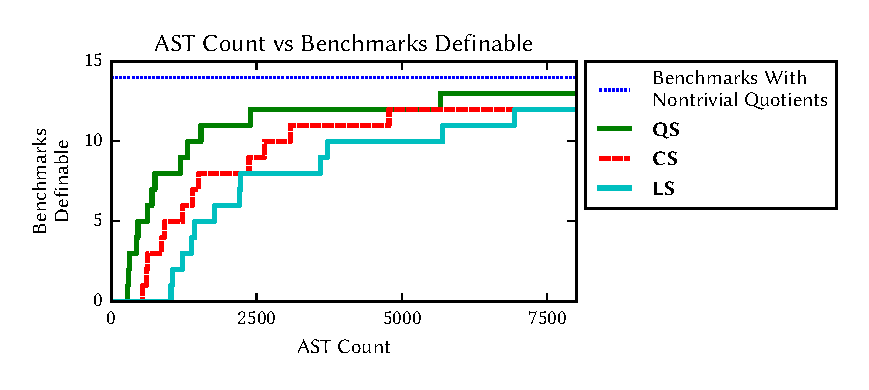
\includegraphics{generated-graphs/asts.eps}
\caption{Count of benchmark programs definable using a given AST count. We find
  that it takes far fewer AST nodes to define benchmark lenses in \Name{} than
  with Optician or without synthesis. }
\label{fig:asts}
\end{figure}

To test if our tool eases the development process, we compare the following
number of AST nodes.
%
\begin{itemize}
  \item[\QRESize{}] \QRESize{} is the number of AST nodes in the QRE
  specifications involved in QRE lens synthesis task.
  \item[\CanonizerAndSpecSize{}] \CanonizerAndSpecSize{} is the number of
  AST nodes in $W(q)$ summed with the number of AST nodes in $\canonizer(q)$,
  for each QRE used in QRE lens synthesis task.
  \item[\LensAndSpecSize{}] \LensAndSpecSize{} is the number of AST nodes
  in $W(q)$ summed with the number of AST nodes in the synthesized QRE lens.
\end{itemize}

The value of \QRESize{} represents the difficulty in writing our benchmarks.

The value of \CanonizerAndSpecSize{} represents the difficulty in writing our
benchmarks without QREs.  This is only an approximation, as both $W(q)$ and
$\canonizer(q)$ are automatically generated from the QRE.  In our
experience, these automatically generated regular expressions and canonizers are
the ones we would naturally write.

The value of \LensAndSpecSize{} represents the difficulty in writing our benchmarks
with neither QREs nor synthesis.  This is also an approximation, as $W(q)$ and
$\canonizer(q)$ and the bijective lens are all automatically generated.
We have found that the generated bijective lens is fairly similar in size to the
one we would manually write, though it is typically less modular.

Figure~\ref{fig:asts} shows the number of benchmarks written with at most a
given number of AST nodes. For a given benchmark, we found \QRESize{} to be
about half as large as \CanonizerAndSpecSize, and about a third as large as
\LensAndSpecSize{}. This demonstrates that introducing QREs saves programmers
significant effort compared to both Optician and basic Boomerang.

\subsection{Increase of Expressivity}

Optician was only able to synthesize fully bijective data transformations.
\Name{} loosens that restriction, and is able to synthesize data which is
bijective when put in canonical form.
To determine the increase of expressivity, we analyzed:
\begin{enumerate}
  \item How many data formats in Optician's benchmark suite required modifications
  to be bijective.
  \item How many data formats in Optician's benchmark suite required modifications
  to be bijective when put in canonical form.
\end{enumerate}

We found that 10 of Opticians 39 benchmarks required modifications to be
bijective. We found that 4 of Optician's 39
benchmarks required modifications to be in bijective correspondence when in
canonical form.  Furthermore, we found that all of the data.gov examples
required no modifications to be in canonical form.  While we did not put the
data.gov examples into a form suitable for Optician, we found only 4 of
the 8 data.gov examples did not require canonization, so making suitable
for Optician would have required a modification of 4 of the data.gov
formats.

\subsection{Competitive Performance}

\begin{figure}
\centering
\begin{subfigure}[b]{.49\textwidth}
\centering
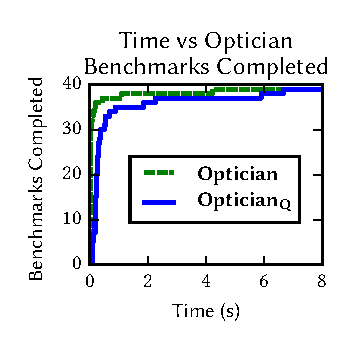
\includegraphics{generated-graphs/times_opt}
\caption{}
\label{subfig:lenssize}
\end{subfigure}
\begin{subfigure}[b]{.49\textwidth}
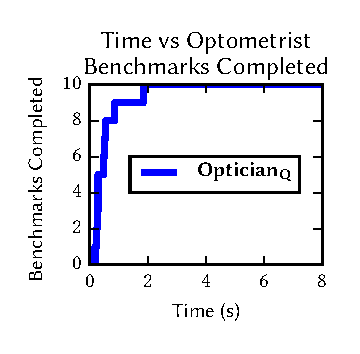
\includegraphics{generated-graphs/times_new.eps}
\caption{}
\label{subfig:examplesused}
\end{subfigure}
\caption{Runtimes of Optician and \Name{}.
In (a), we run Optician and \Name{} on Optician's benchmarks.  We find that
there is only a negligible difference incurred by Optometrist's overhead.
In (b), we run Optometrist on its benchmark suite.  We find that it is able
to synthesize all quotient lenses in under 20 seconds, and typically
finished in under 5 seconds. }
\label{fig:times}
\end{figure}

While we expanded on the Optician system, we found it important to validate
performance did not degrade in this expansion.  To validate this, we tested:
\begin{itemize}
  \item[\OpticianRuntime{}] Optician runs on its own benchmarks.
  \item[\SystemOnOptician{}] \Name{} runs on Optician's benchmarks.
  \item[\SystemOnBenchmarks{}] \Name{} runs on its own benchmarks.
\end{itemize}

We summarize the results of these experiments in Figure~\ref{fig:times}.
\Name{} was
able to synthesize all of Optician's benchmarks at a speed competitive with
Optician.  There was additional overhead in calculating $W(q)$ and $K(q)$,
resulting in a very slight decrease in performance.

Also notable was one of the data.gov examples, which converted demographic
statistics by zip code from xml form into rdf form.  This merely took longer because it was
an exceptionally large format, converting over 40 fields.  After adding in additional
fields to make this format bijective, it still took over 15 seconds to complete.

\section{Related Work}
\label{relwork}

\iffalse
Bidirectional transformations have been used in diverse areas of computing
where they arise as parsers and pretty printers, marshallers
and unmarshallers, serializers and deserializers, database views and view
updaters and many others\sam{TODO put citations}. Such transformations have
been extensively studied since they were proposed as a solution to the classical
{\em view-update problem} in the database community, where the challenge is to
derive a program that extracts a view of data from a source, as well as a
program that folds view updates back into the source safely and correctly.
\fi
This paper builds on the work of Foster et al~\cite{quotientlenses} who
introduced the theory of quotient lenses and implemented quotient lenses as a
refinement of the bidirectional string processing language Boomerang.
In Boomerang, the source and target types are specified using regular
expressions, and the equivalence relations are expressed using canonizers, which
are functions that map elements of a regular language to their canonical
representative. Boomerang canonizers can express a very broad class of
equivalence relations between regular languages, but actually doing so is often
difficult with complicated equivalence relations. For instance, Boomerang's
in-build permutation combinator does not account for separators in between the
regular expressions. Also, this combinator permutes regular expressions rather
than canonizers, thus making it difficult to express nested permutations that
occur in many data formats, especially XML and XML-like formats.

In their paper, Foster et al also discuss other bidirectional programming
languages that support quotienting of data including XSugar~\cite{xsugar},
biXid~\cite{bixid} and X/Inv~\cite{Hu2004,Mu2004,Mu2006}. XSugar programs
bidirectionally convert data stored in XML and ASCII formats respectively, with the
transformations specified by a pair of unambiguous grammars. The quotienting
occurs on the XML side by use of a generic canonizer that standardizes the
representation of trees. Well-formed XSugar programs are guaranteed to be
bijective modulo an equivalence relation that captures XML normalization. biXid
programs convert between pairs of XML documents, with the XML formats specified
using a pair of grammars as in XSugar. However, biXid grammars can be ambiguous.
This ambiguity is what allows biXid to express equivalences on the data.
Finally, Foster et al discuss a possible connection with the languages
X and Inv which support a primitive duplication combinator that does not work
well with the lens laws, but can be expressed using Boomerang quotient lenses.

As far as synthesis goes, though there is a good deal of recent research on
synthesizing unidirectional string
transformations~\cite{singh2012learning,le-pldi-2014,gulwani-popl-2014,perelman2014test,Singh:blinkfill},
the system Optician, which we introduced in ~\cite{optician}, is the first attempt
to synthesize bidirectional transformations that we are aware of. In that
publication, we compared Optician to two of these unidirectional string
transformers, Flash Fill~\cite{gulwani-popl-2014} and
FlashExtract~\cite{le-pldi-2014}, and found that these tools were unsuccessful
in synthesizing the complex transformatiunons that can be expressed in Optician.

While Optician improved on prior effors at synthesizing unidirectional string
transformers and introduced synthesis for bidirectional string transformations,
Optician was only able to synthesize fully bijective data transformations. Our
new system \Name{} improves on Optician in that \Name{} loosens this
restriction, and is able to synthesize data which is bijective when put in
canonical form. \Name{} is therefore a refinement of Optician since the
new synthesis algorithm (i.e. the quotient lens synthesis algorithm) restricted
to ``pure'' regular expressions degenerates to the synthesis algorithm that
we introduced in Optician. Indeed, as we mentioned in the evaluation section,
\Name{} was able to synthesize all of Optician's benchmarks at a speed
competitive with Optician, though there was additional overhead in calculating
the whole language $W(c)$ and the kernel language $K(c)$ of QREs, which
resulted in a very slight decrease in performance.

Much of the research in synthesis assumes that the synthesizer is provided with
a collection of examples. Optician and Optometrist differ in that they requires
that the programmer supplies both examples {\em and} format descriptions in the
form of regular expressions or QREs.  There is a trade-off here.  On the one
hand, a user must have some programming expertise to write regular expression
(or QRE) specifications and it requires some work. On the other hand, such
specifications provide a great deal of information to the synthesis system,
which decreases the number of examples needed (often to zero), makes the system
scale well, and allows it to handle large, complex formats.  By providing these
format specifications, the synthesis engine does not have to both infer the
format of the data as well as the transformations on it, obviating the need to
infer tricky formats like those involving nested iterations. Furthermore, by
focusing on bidirectional transformations, we limit the space of synthesized
functions to bijective ones, reducing the search space, and the expressiveness
of the search space.

There are many other recent results showing how to synthesize functions from
type-based
specifications~\cite{augustsson-2004,osera+:pldi15,feser-pldi-2015,scherer-icfp-2015,frankle+:popl16,armando+:pldi16}.
These systems enumerate programs of their target language, orienting their
search procedures to process only terms that are well-typed.
Optician is distinctive in that it synthesizes terms in a language with many
type equivalences.
Perhaps the system most similar to Optician is InSynth~\cite{gvero-pldi-2013}, a
system for synthesizing terms in the simply-typed lambda calculus that addresses
equivalences on types. Instead of trying to directly synthesize terms of the
simply-typed lambda calculus, InSynth synthesizes a well-typed term
in the succinct calculus, a language with types
that are equivalent ``modulo isomorphisms of products and
currying''~\cite{gvero-pldi-2013}. The type structure that we used in Optician
is significantly more complex.  In particular, because Optician types do not
have full canonical forms, we used a pseudo-canonical form, which captures part
of the equivalence relation over types. To preserve completeness, we pushed
some of the remaining parts of the type equivalence relation into a set of
rewriting rules and other parts into the synthesis algorithm itself.

Morpheus~\cite{morpheus} is another synthesis system that uses two
communicating synthesizers to generate programs.  In both Morpheus and
Optician, one synthesizer provides an
outline for the program, and the other fills in that outline with program
details that satisfy the user's specifications.
This approach works well in large search spaces that require some enumerative
search.
One important way that Optician differs from Morpheus is that in
Morpheus, an outline is a sketch---an
\emph{expression}
containing holes---whereas
an outline in Optician is a pair of regular
expressions, i.e., a
\emph{type}.  Moreover, in order to implement an efficient
search procedure, we had to create both a new type language and a new
term language for lenses.  Once we did so, we proved our new, more
constrained language
designed for synthesis was just as expressive as the original, more
flexible and compositional language designed for human programmers.


\section{Conclusion and Future Work}
\label{concl}

\bibliographystyle{plain}
\bibliography{local}


\end{document}
